% ######################################################################################################################
%         PhAT
% ######################################################################################################################

% \chapter{Phylogenetic Automatic (Reference) Trees}
%Preparatory and

\chapter{Ancillary Methods for Phylogenetic Placement}
\label{ch:AutomaticTrees}

\paperbox{
    This chapter is based on the peer-reviewed publication:
}{\paperart}{
    \textbf{Contributions:} Lucas Czech... Pierre Barbera... Alexandros Stamatakis... and...
}

% ######################################################################################################################
%     Background and Motivation
% ######################################################################################################################

\section{Background and Motivation}
\label{ch:AutomaticTrees:sec:Motivation}

Molecular sequencing costs are decreasing exponentially, leading to unprecedented amounts of genetic sequence data,
as explained in \secref{ch:Foundations:sec:SequenceAnalysis:sub:Metagenomics}.
In most metagenomic studies, an initial analysis step consists in assessing the evolutionary provenance of the sequences.
Phylogenetic placement, as introduced in \secref{ch:Foundations:sec:PhylogeneticPlacement},
can be employed to determine the evolutionary position of sequences with respect to a given reference phylogeny.

This is particularly helpful for studying new, unexplored environments,
for which no closely related sequences exist in reference databases yet \cite{Mahe2017}.
However, the selection process of suitable reference sequences
for inferring a reference tree is typically conducted manually.
This constitutes a major challenge and hindrance for studying such environments with placement methods.

This limitation also concerns the use of phylogenetic placement for taxonomic assignment.
In studies that specifically look for certain kinds of organisms, e.g, protists \citep{Mahe2017},
it usually suffices to use a taxonomy covering the organisms of interest,
potentially including outgroups from more distantly related species.
As metagenomic analyses get cheaper,
it is however to be expected that researchers want to target more than one group of organisms within one study.
Particularly in cases where the environment contains a yet unknown diversity of organisms,
this hence necessitates to use a broad reference that covers many taxonomic clades.
At the same time however, the number of taxa in the reference phylogeny
should be small enough to allow for visually inspecting and interpreting the results.

Lastly, phylogenetic placement methods have generally already reached their scalability limits:
They require a higher computational effort with respect to the placement algorithms \emph{per se},
but also the pre- and post-processing, than, for instance, similarity-based methods such as \toolname{BLAST}.

% Due to the continuous advances in molecular sequencing, existing placement methods
% as well as respective pre- and post-processing tools have already reached their scalability limits.

% ######################################################################################################################
%     Methods
% ######################################################################################################################

\section{Methods}
\label{ch:AutomaticTrees:sec:Methods}

% First, we introduce a method to automatically construct representative sequences from databases to infer reference phylogenies.
% Second, we present an approach for conducting large-scale phylogenetic placements on nested phylogenies.
% Third, we describe a preprocessing pipeline that allows for handling huge sequence data sets.
% Our experiments on empirical data show that our methods substantially accelerate the workflow and
% yield highly accurate placement results.

Here, we introduce methods to overcome the aforementioned limitations, that is, to
(1) automatically obtain a high-quality reference tree for conducting phylogenetic placement,
(2) split up the placement process into two steps using smaller phylogenies,
and (3) accelerate the computation of placements via appropriate data pre-processing approaches.
All methods are implemented as part of our \toolname{gappa} tool;
see \appref{ch:PipelineImplementation} for implementation details.
% which is freely available under GPLv3 at \url{http://github.com/lczech/gappa}.

% ======================================================================================================================
%     Phylogenetic Automatic (Reference) Trees
% ======================================================================================================================

\subsection{Phylogenetic Automatic (Reference) Trees}
\label{ch:AutomaticTrees:sec:Methods:sub:PhAT}

\paragraph{Motivation}
\label{ch:AutomaticTrees:sec:Methods:sub:PhAT:par:Motivation}

Molecular environmental sequencing studies, particularly those that aim to conduct phylogenetic placement of \acfp{QS},
often rely on a set of manually selected and aligned reference sequences
to infer a \acf{RT} \cite{Tedersoo2014,DeVargas2015,Mahe2017,Thompson2017}. % references thanks to Micah!
% \cite{Stoeck2010,Srinivasan2012,Dunthorn2014,Mahe2017}.
%as a frame in which their data are analyzed and interpreted.
Creating and maintaining databases of such reference sequences constitutes a labor-intensive and potentially error-prone process.
Moreover, this approach is impractical for highly diverse samples that comprise sequences from many taxonomic clades,
or samples obtained from unexplored environments, where it is yet unknown which reference sequences are necessary.
Lastly, even if a large \ac{RT} is available,
the visualization of placements on such an \ac{RT} might be confusing and thus hard to interpret.

The \ac{RT} used for phylogenetic placement should ideally
(a) cover all major taxonomic groups that occur in the \acp{QS},
(b) use high-quality error-free reference sequences, and
(c) not be too large to allow for unambiguous visualization and interpretation.
These criteria can be met for small datasets by manually selecting curated sequences from databases,
potentially informed by literature describing these sequences.
In order to increase coverage, often additional sequences are selected
based on their similarity to the already selected ones.
For large and taxonomically diverse samples one key challenge is that sequence databases such as
\toolname{Greengenes} \cite{DeSantis2006}, \toolname{Unite} \cite{Abarenkov2010}, \toolname{PR2} \cite{Guillou2012},
\toolname{EzTaxon} \cite{Kim2012}, \toolname{Silva} \cite{Quast2013}, and \toolname{RDP} \cite{Cole2014}
maintain reference collections of thousands to millions of taxonomically annotated sequences.
Therefore, one needs to appropriately sub-sample sequences such that the \ac{RT}
can be inferred in reasonable time {\em and} sufficiently covers the diversity of the sample.

Previous approaches mainly relied on phylogenetic diversity
\cite{Faith1992,Pardi2005,Minh2006} and related methods \cite{Matsen2013}.
The major drawback is that they require a comprehensive phylogeny as input.
%While using the evolutionary information of a tree is generally reasonable,
%it might be impractical for selecting reference sequences.
% One has to select a set of comprehensive sequences, infer their phylogeny, and only then is able to select the actual ref seqs
Inferring such large comprehensive phylogenies with hundreds of thousands of taxa,
to subsequently reduce the taxon set again, is computationally inefficient and in certain cases infeasible.
% One first has to infer a phylogeny for a potentially large set of candidate sequences,
%which is not always feasible,
% if the list of candidate sequences is too large to build a comprehensive tree,
%only to then squeeze it down to the actual number of desired reference sequences.

% We present an approach that eliminates the need for a hand-crafted database of suitable reference sequences.
To this end, we present a computationally efficient approach
for obtaining sequences from large databases to infer an \ac{RT}.
This \ac{RT} is then used for conducting phylogenetic placement analyses.
The input of our method is a database of aligned sequences of known species, including their taxonomic labels.
Our approach then identifies sets of sequences that are similar to each other based on their entropy.
It subsequently reduces the sequences in these sets to a predefined number of consensus sequences.
This set of sequences is the output of our method.
It represents the taxonomic clades and is then used to infer the \ac{RT}.

% ======================================================================================================================
%     Sequence Entropy
% ======================================================================================================================

% \subsection{Sequence Entropy}
% \label{ch:AutomaticTrees:sec:Method:sub:SequenceEntropy}

\paragraph{Sequence Entropy}
\label{ch:AutomaticTrees:sec:Methods:sub:PhAT:par:SequenceEntropy}

Conventional methods for sequence similarity are often based on edit distance
and other pairwise comparison methods \cite{Needleman1970,Smith1981,Altschul1990}.
This however necessitates to transform the pairwise distances to some form of ensemble measure
that describes the similarity of all sequences to each other, for which there is no obvious approach \cite{Zhou2006}.
There also exist methods that describe genetic variation and
nucleotide diversity of sets of sequences \cite{Nei1979,Blaisdell1986} which could be used for this purpose.

We here use entropy \cite{Shannon1951} to define a measure
for quantifying the ensemble similarity of a set $s$ of sequences.
% We here use entropy for measuring ensemble similarity of a set of sequences.
% We define a measure to quantify the ensemble similarity of a set $s$ of sequences,
% based on their entropy \cite{Shannon1951}.
% We use the per-site entropy of $s$ to calculate a similarity score for the whole set.
% In order to quantify the similarity of a set $s$ of aligned sequences, we use the per-site entropy of $s$.
Variants of sequence entropy have been used before in numerous biological and phylogenetic contexts,
for example, to asses the information content of sequences
% Can probably remove a few of those references... first, the full list, later, the most important ones
\cite{Schmitt1997,Vinga2003,Vinga2004,Li2005,Criscuolo2010,Comin2012,Vinga2014},
or to measure substitution saturation \cite{Xia2003}.
Here, we use entropy for alignment sites, that is, we define the entropy (uncertainty) $H$ at alignment site $i$ as
%shown in \eqnref{eq:entropy}.

\begin{equation}
    \label{ch:AutomaticTrees:eq:entropy}
    H_{i} ~=~ -\sum_c f_{c,i} \times \log f_{c,i}
\end{equation}

where $c \in \left\{ \texttt{A}, \texttt{C}, \texttt{G}, \texttt{T}, \texttt{-} \right\}$ is the set of nucleotide states
including gaps, and $ f_{c,i} $ is the frequency of character $c$ at site $i$ of the alignment.
% The relative frequency is calculated using the characters of all sequences in the set.
Including gaps (\texttt{-}) in the summation reduces the contribution of sites that contain a large fraction of gaps.
Their contribution is weighed down as all standard phylogenetic inference tools model gaps as undetermined states,
that is, they do not contribute anything to the likelihood score.
The entropy is \num{0} for sites that only contain a single character.
It increases the more different characters an alignment site contains, {\em and} the more similar their frequencies are.
% low for sites with one dominant character, and high for sites with a similar distribution of more than one character.
Its maximum occurs if all characters appear with the same frequency (each of them \num{20}\%).
Note that we also treat ambiguous characters as gaps
(see \secref{ch:Foundations:sec:SequenceAnalysis:sub:ConsensusSequences}).
As only \num{0.008}\% of the non-gap characters in our test database (\toolname{Silva}) are ambiguous,
their influence is negligible.
Ambiguous characters could however be incorporated by using fractional character counts.

Finally, the total entropy of a set $s$ of aligned sequences is simply the sum over all per-site entropies:
$H(s) = \sum_i H_i$.
% By dividing this value by the length of the alignment, the measure becomes comparable across alignments.
It is also possible to normalize this value by dividing it by the length of the alignment
to get comparable values across alignments.
Here, this however does not make a difference, as we are always comparing sequences with the same alignment length.
We use this entropy to quantify the ensemble similarity of a set of sequences.
This can be regarded as an information content estimate of the sequences.

% ======================================================================================================================
%     Sequence Grouping
% ======================================================================================================================

% \subsection{Sequence Grouping}
% \label{ch:AutomaticTrees:sec:Method:sub:SequenceGrouping}

\paragraph{Sequence Grouping}
\label{ch:AutomaticTrees:sec:Methods:sub:PhAT:par:SequenceGrouping}

The goal of this step is to group the sequences of a database into a given target number of groups/sets,
such that the groups reflect the diversity of the sequences in the database.
At the same time, the number of sequences needs to be small enough
such that a maximum likelihood \ac{RT} can be inferred in reasonable time.

A possible approach would be to use agglomerative clustering:
In each step, the sequences that have the lowest entropy are clustered
until the desired number of reference sequences is reached.
A supposed advantage of this approach is that it does not rely on any taxonomic information
(in contrast to our approach presented below).
This procedure is however computationally expensive, having a complexity in $\mathcal{O}(n^2\log n)$,
and is thus not applicable to large databases with millions of sequences.
Furthermore, the resulting sequence clusters can generally not be assigned unambiguous taxonomic labels,
that is, they lack an interpretable naming scheme.
This severely limits the types of useful post-analyses that can be executed;
we did therefore not explore this approach.

Instead, we use the taxonomic information (see \secref{ch:Foundations:sec:TreeOfLife:sub:TaxonomyNomenclature})
of the sequence database to identify potential candidate groups of sequences
that could be represented by a consensus sequence (see \secref{ch:Foundations:sec:SequenceAnalysis:sub:ConsensusSequences}).
We interpret a taxonomy as a sequence labeling, where similar sequences have related labels.
Thus, a taxonomy represents a pre-classification of similar sequences that can be exploited to group them.
% However, this assumes that the taxonomic classification is correct for most sequences \cite{Kozlov2016}.
% The impact of taxonomic mislabels and spurious sequences is absorbed by using consensus sequences.

\begin{figure}[t!hpb]
    \centering
    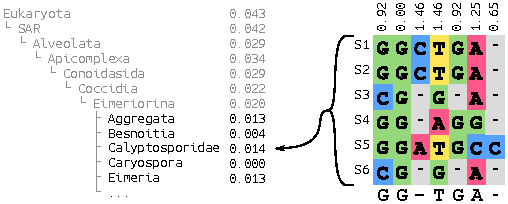
\includegraphics[width=0.8\linewidth]{art/tax_entropy.pdf}
    \caption[Entropy and consensus sequence of a taxonomic clade]{
        \textbf{Entropy and consensus sequence of a taxonomic clade.}
        The left hand side shows the exemplary clade \taxonname{Eimeriorina} in its taxonomic context,
        listing its super- and sub-clades with the normalized entropy of their respective sequences.
        The right hand side is an excerpt from the alignment
        of six sequences that belong to the \taxonname{Calyptosporidae} sub-clade.
        At its top, the per-site entropies for the alignment columns are shown.
        At the bottom, the majority rule consensus sequence is shown, which is used to represent the sub-clade.
    }
    \label{fig:tax_entropy}
\end{figure}

For a clade $t$ of the taxonomic tree, we denote by $H(t)$ the entropy of all sequences that belong to that clade,
including all sequences in its sub-clades, that is, its lower taxonomic ranks.
Clades with low entropy imply that they contain highly similar sequences that can in turn be represented
by a consensus sequence without sacrificing too much diversity.
Inversely, clades with high entropy contain diverse sequences,
implying that a consensus sequence is not likely to sufficiently capture the inherent sequence diversity.
It is thus better to expand these clades and construct separate consensus sequences for their respective sub-clades.
An example is shown in \figref{fig:tax_entropy}.
As the clade structure of a taxonomy forms a tree, this criterion can then be applied recursively,
as shown in \algref{algo:taxonomy_expansion}.

\todo{the formatting is currently off here...}

\begin{algorithm}
\caption{\textbf{Taxonomy Expansion}}\label{algo:taxonomy_expansion}
\begin{algorithmic}[1]
%     \State \textbf{Input:} $\text{Taxonomy } T$
%     \State \textbf{Input:} $TargetCount$
    \State $ \textit{Candidates}  \gets \text{list of highest ranking clades}$
    \State $ \textit{TaxaCount} \gets \text{size of } \textit{Candidates} $
    \While{ $ \textit{TaxaCount} < \textit{TargetCount} $ }
        \State $ \textit{MostDiverse} \gets \argmax_{~t \in \textit{Candidates}~} H(t) $
        \State remove $\textit{MostDiverse}$ from $\textit{Candidates}$
        \State add \text{sub-clades of }$\textit{MostDiverse}$ to $\textit{Candidates}$
        \State $\textit{TaxaCount} \gets \textit{TaxaCount} - 1 + \text{size of } \textit{MostDiverse}$
    \EndWhile
    \State \textbf{return} $\textit{Candidates}$
\end{algorithmic}
\end{algorithm}

The algorithm works as follows:
We initialize a list of candidate clades with the highest ranking clades that we want to consider.
In the most general case, these can be ``Archaea'',  ``Bacteria'', and ``Eukaryota''.
%but the narrower the clade, the more accurate the result.
We then select the most diverse candidate clade, that is,
the clade $t$ whose sequences exhibit the highest entropy $H(t)$.
This clade is then expanded,
and we do not consider it as a potential candidate for building a consensus sequence.
The high entropy clade is then removed from our list and its immediate sub-clades are added as new candidates to the list.
Finally, the current count of how many candidates we have already selected is updated accordingly.
By expanding clades with high entropy, we descend into the lower ranks of the taxonomy.
On average, this decreases the entropy,
because low ranking clades generally tend to contain more similar sequences.
% Thus, we obtain a list of candidate clades that have a low entropy, i.e., similar sequences.
This process is repeated until our list contains approximately as many candidate clades
as the desired target count of reference sequences, which is provided as input.
As the sizes of expanded clades can vary substantially, the target count cannot always be met exactly.
In our tests, the average deviation was \num{0.2}\%, as shown later in \tabref{tab:TaxonomicComposition}.
% Because of differently sized clades, the algorithm can yield some more sequences than requested.

%Remark: Clades can have different sizes, that is, contain different number of sequences.
%It thus can happen that the algorithm yields some more sequences than requested.
%Furthermore, when calculating the entropy of a clade that contains large sub-clades with low entropy,
%the contribution of small sub-clades with high entropy can vanish.
%This effect can be minimized by using a larger target count.
% \todo{Do we need some extra evaluation of this? I think, the general accuracy numbers are sufficient,
% but maybe we find a way of quantifying this effect a bit more.}
% \todo{I'm not happy with the place of the above paragraph in the text. Maybe it should go somewhere else.}

%%An alternative stopping criterion is to use an entropy threshold,
%hat is, we expand as long as the sequence entropy is above this threshold.
%There is however no intuitive threshold value to use, thus the target count criterion is easier to work with.
%\todo{This paragraph can totally be left out.}

Given this list of clades from different taxonomic ranks, we can now compute the consensus sequences.
% As the clades were selected to have a low entropy, they contain sequences that are similar to each other.
For each clade, all sequences in that clade and its sub-clades are used to construct a consensus sequence,
which represents the clade diversity, and serves as the reference sequence for that clade.
This has several advantages:
If only a few sequences diverge from the majority of that clade,
the entropy might underestimate the molecular diversity of a clade.
The consensus sequence for such a clade however compensates for this.
Using consensus sequences furthermore levels out spurious and erroneous sequences in the database.
A simple per-site majority rule consensus \cite{May1952,Day1992a} works well,
but we also assessed alternative methods;
see \figref{fig:consensi_backbone} and \figref{fig:single_seqs} for details.

The algorithm can start at any rank of the taxonomy in order to only group sequences from specific clades.
It is computationally cheap compared to pairwise sequence comparison,
while still yielding reasonable representative sequences for large taxonomic clades.
Note that it would also be possible to directly use the relative character frequencies at each site
to obtain more accurate representations.
Maximum likelihood-based phylogenetic inference tools do, in principle, not require discrete input sequences,
as explained in \secref{ch:Foundations:sec:MLTreeInference:sub:LikelihoodComputation}.
The likelihood model allows to account for uncertainty in the input data \cite{Felsenstein2004},
although this is generally not implemented in the mainstream software packages.
%However, current implementations of the phylogenetic placement do not support this information yet.
The above process yields a set of consensus reference sequences which capture the diversity of distinct taxonomic clades.

% ======================================================================================================================
%     Inferring Reference Trees
% ======================================================================================================================

% \subsection{Inferring a Reference Tree}
% \label{ch:AutomaticTrees:sec:Method:sub:ReferenceTrees}

\paragraph{Inferring a Reference Tree}
\label{ch:AutomaticTrees:sec:Methods:sub:PhAT:par:InferringReferenceTree}

%Once the sequence grouping is completed, the taxonomy is not longer needed.
% Note that the taxonomy is not longer used at this point.
Once we have identified the consensus sequences, which are already aligned to each other,
we can use them to infer a maximum likelihood tree, which we call a \emph{Phylogenetic Automatic (Reference) Tree} (PhAT).
\acused{PhAT}
As each consensus sequence is associated with a taxonomic clade,
the corresponding taxonomic path can be used to label the tips of the tree.
Note that since clades with low entropy might not be expanded,
the tip labels do not necessarily correspond to species or genus level.
Also, the \ac{PhAT} will not necessarily be congruent to the taxonomy,
unless the tree search is specifically constrained in that way
(see \secref{ch:Foundations:sec:MLTreeInference:sub:FurtherAspects:par:ConstrainedTrees}).

A \ac{PhAT} satisfies all criteria we listed above:
(a) All taxonomic groups occurring in the \acp{QS} can be covered by using a suitable taxonomy as input.
(b) By using consensus sequences, potential sequencing errors can be alleviated.
(c) The size of the tree can be specified by the user.
However, the resolution of the trees is limited by the underlying taxonomy,
see \secref{ch:AutomaticTrees:sec:Evaluationsub:EmpiricalDatasets}
and \secref{ch:AutomaticTrees:sec:Evaluation:sub:TaxonomicAssignmentProfiling} for details.
Thus, one needs to verify that the resulting tree is appropriate for the dataset to be placed on it.
This however also holds for manually selected reference sequences,
and is hence not a specific disadvantage of our method.
Furthermore, using consensus sequences may obscure the degree of sequence diversity in sub-clades,
which in turn can affect the accuracy of subsequent phylogenetic placements on that tree.
Our algorithm as described here can not fully compensate for this.
We present a method to address both issues (tree resolution and obscured diversity) in the next Section.
% The usage of these trees however has limitations.
% For a discussion, see Section~\ref{sec:DiscussionConclusion}.

% ======================================================================================================================
%         Multilevel Placement
% ======================================================================================================================

\subsection{Multilevel Placement}
\label{ch:AutomaticTrees:sec:Methods:sub:MultilevelPlacement}

% \paragraph{Motivation}
% \label{ch:AutomaticTrees:sec:Methods:sub:MultilevelPlacement:par:Motivation}

When conducting phylogenetic placement, the computationally limiting factors are
(i) the number of \acp{QS} to be placed (addressed in the following \secref{ch:AutomaticTrees:sec:Methods:sub:DataPreprocessing})
and (ii) the size of the \ac{RT} (number of taxa) and corresponding alignment length (addressed here).
% This section addresses a way to work with large number of reference sequences,
% while the next section explains how to deal with large number of query sequences.
Using \acp{RT} with more taxa increases the phylogenetic resolution of the placements,
at the cost of increased computational effort for inferring the \ac{RT}, aligning the \acp{QS}, and placing the \acp{QS}.
Furthermore, longer reference alignments (if appropriate data is available)
are required to accurately infer large trees under the maximum likelihood criterion \citep{Yang1994},
thus further increasing the computational costs.
Lastly, placement on large trees that comprise reference sequences with high evolutionary distances
can reduce placement accuracy \citep{Mirarab2012}.
% It is hence impractical and unfavorable to employ reference trees with more than a few thousand taxa.
Thus, using a large number of reference sequences is not always desirable in practice.

One solution is to divide the tree and its alignment into more conquerable subsets, % pun intended
for example as implemented in \toolname{SAT\'{e}} \citep{Liu2009,Liu2012}.
% which is a method that simultaneously improves an alignment and the tree inferred from it.
This approach has also been extended to phylogenetic placement
in \toolname{SEPP} \citep{Mirarab2012} and \toolname{TIPP} \citep{Nguyen2014},
which divide the tree into disjoint subsets of taxa and conduct placement on each of them.
While yielding more accurate placements and taxonomic classifications in less computing time,
this method might still result in large reference trees, which are hard to inspect and visualize.

% \paragraph{Method Description}
% \label{ch:AutomaticTrees:sec:Methods:sub:MultilevelPlacement:par:Multilevel}

To address this issue, we present an approach called \emph{Multilevel} or \emph{Russian Doll} Placement,
which is summarized in \figref{fig:multilevel_placement}.
% It integrates well with the previously described Automatic Reference Tree method.
Instead of working with one large \ac{RT} comprising {\em all} taxa of interest,
we use a smaller, but taxonomically broad \ac{BT} for pre-classifying the \acp{QS} (first level),
and a set of refined \acp{CT} for the final, more accurate placements (second level).
These \acp{CT} comprise the reference sequences that are of interest for a particular study.
For example, if a study is concerned with \taxonname{Apicomplexa} and \taxonname{Cercozoa},
a broad \taxonname{Eukaryotes} \ac{BT} can be used for the first level,
and two respective \acp{CT} for the second level, in analogy to \citep{Mahe2017}.
% The decisions about which \acp{CT} are needed to represent the \acp{QS} of a study,
% which reference sequences to use for the \ac{BT} and \acp{CT},
% and which branches of the \ac{BT} represent a \ac{CT}
% are up to the design of the study.
Each \ac{CT} is associated with the set of branches of a specific \ac{BT} clade.

\begin{figure}[hpbt]
    \centering
    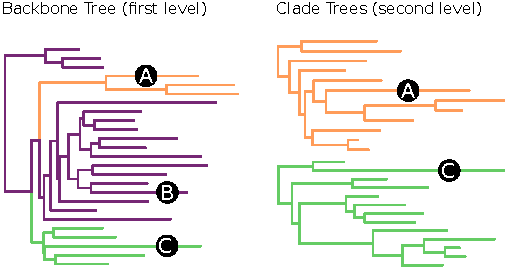
\includegraphics[width=0.75\linewidth]{art/multilevel_placement.pdf}
    \caption[Multilevel Placement]{
        \textbf{Multilevel Placement.}
        The left shows a backbone tree (BT); the right shows two clade trees (CTs) in orange and green.
        Branches in the BT that are associated with a CT are marked in its color.
        The trees ``overlap'' each other, meaning that each CT is represented by multiple branches in the BT.
        Three sequences {\sffamily A}, {\sffamily B}, and {\sffamily C} are placed on the BT, which is the first level.
        {\sffamily A} and {\sffamily C} are placed on branches associated with a CT.
        Hence, their second level placement is conducted on the respective CT.
        {\sffamily B} is placed on a branch that is not associated with any CT,
        and thus not used in the second level.
    }
    \label{fig:multilevel_placement}
\end{figure}

The method then works in three steps:

\begin{enumerate}
    \item Align and place the \acp{QS} using the \ac{BT} (first level).
    \item For each \ac{CT}, collect the \acp{QS} that are placed on the \ac{BT} branches associated with the \ac{CT}.
    \item Align and place these \acp{QS} again, using their specific \acp{CT} (second level).
\end{enumerate}

While this approach requires some additional bookkeeping,
the total computational cost is reduced,
because the \acp{QS} do not have to be placed on all branches of all \acp{CT}.
The speed gain depends on the sizes of the \ac{BT} \emph{and} the \acp{CT}
with respect to the size of the substantially larger (often one order of magnitude or more) comprehensive tree.
For example, by splitting a tree with \num{10 000} taxa into a \ac{BT} and \num{10} \acp{CT} with 1000 taxa each,
the computational cost decreases by a factor of 5 (two placement levels with 10\% of the cost each).
Furthermore, at each level,
the amount of required computer memory is reduced by a factor of \num{10} compared to the large tree.
Lastly, this method allows for fine-grained control over the clades of interest at both placement levels:

Firstly, the \ac{BT} provides a means for phylogenetically informed sequence filtering---%
that is, to identify and remove ``spurious'' \acp{QS}.
Sequences with low similarity to known references are often removed in environmental sequencing studies \citep{Stoeck2010}.
However, using sequence similarity as a filter criterion can remove too many \acp{QS},
particularly when studying new, unexplored environments \citep{Mahe2017}.
By using phylogenetic placement as a filter instead, substantially more sequences can be retained for downstream analyses.
Only the \acp{QS} that are placed onto the inner branches of the \ac{BT},
that is, branches with no associated \ac{CT},
are omitted at the second placement level.
Such placements may indicate that suitable reference sequences are missing from the \ac{RT},
or that the respective \acp{QS} represent novel species.
Either way, as these \acp{QS} are not well represented by the \ac{RT},
they are not informative for most downstream analyses and can thus be removed.
This thus represents a phylogenetically informed sequence filtering method as an alternative to sequence similarity.
% See also Section \nameref{sec:Postprocessing:sub:Visualization}.
% We applied a similar approach before % (using manually selected reference sequences)
% in order to work with \acp{QS} which were not covered well in reference databases \citep{Mahe2017}.
% \todo{Damn, I keep on citing our paper over and over again... we already did everything in there!}
% \todo{Also, the sentence can also be left out -- the paper was already cited three sentences ago.}

Secondly, using specific clade trees for lower level taxonomic clades offers the phylogenetic resolution
that is necessary for downstream analyses and for biological reasoning.
It is, for example, possible to use manually curated ``expert'' trees for each clade of interest.
% This approach is currently being tested in the context of the \toolname{UniEuk} project \citep{Berney2017}.

In this setup, the \ac{BT} is only used for pre-classification,
and can, for example, use our \ac{PhAT} method as presented in \secref{ch:AutomaticTrees:sec:Methods:sub:PhAT}.
The aforementioned issue of obscured diversity in sub-clades can be circumvented
by ``overlapping'' the \acp{CT} with the \ac{BT}.
That is, a \ac{CT} can be associated with several branches of the \ac{BT},
so that placements on each of these \ac{BT} branches are collected and placed onto the same \ac{CT}.
See \figref{fig:multilevel_placement} and \figref{fig:clades} for examples.
We recommend to ensure that the branches of the \ac{BT} that are associated with one \ac{CT} are monophyletic,
meaning that there is one split that separates these branches from the rest of the \ac{BT}.
This can be achieved by inferring the \ac{BT} with a high-level constraint that maintains the monophyly of the \acp{CT}.
It ensures phylogenetic consistency between the \ac{BT} and the \acp{CT},
and improves the accuracy of the first placement level,
as shown in \secref{ch:AutomaticTrees:sec:Evaluation:sub:MultilevelPlacement}.
% It can be achieved by inferring the \ac{BT} with a high-level constraint.
% that is, constraining the reference sequences that map to a \ac{CT} to be monophyletic.
% This constraint is however not necessary.
Lastly, it is also possible to use more than two levels,
which might become necessary when working with \acp{RT} and datasets even larger than what is currently available.

% ======================================================================================================================
%         Data Preprocessing for Phylogenetic Placement
% ======================================================================================================================

\subsection{Data Preprocessing for Phylogenetic Placement}
\label{ch:AutomaticTrees:sec:Methods:sub:DataPreprocessing}

Apart from the \ac{RT} size, handling the sheer number of \acp{QS}
also induces computational limitations for conducting phylogenetic placements.
Most metagenomic studies publish their data in unprocessed formats,
which are sometimes filtered to contain only reads from certain barcoding or marker regions.
For instance, they store the raw sequencing output in \fileformat{fasta} \citep{Pearson1988}
or \fileformat{fastq} \citep{Cock2009} format (see \secref{ch:Foundations:sec:SequenceAnalysis:sub:GenomeSequencing}).
Those data often contain duplicates of exactly identical sequences, both {\em within} and {\em across} samples.
% As identical sequences are treated exactly the same in phylogenetic placement,
% de-duplication can rigorously reduce the computational cost.
Identical sequences are however treated the same in phylogenetic placement algorithms
and therefore induce unnecessary computational overhead.
Furthermore, sample sizes, that is, the number of sequences per sample, can vary by several orders of magnitude.
For example, the ``HM16STR'' dataset of the \ac{HMP} \citep{Huttenhower2012,Methe2012}
contains an average of \num{12 911} sequences per sample,
but also an outlier sample with \num{0} sequences and one with \num{403 211} sequences.
If the placement algorithm is parallelized over samples, this leads to an uneven load balance across compute nodes.
A potential solution is to initially cluster the sequences into OTUs
(see \secref{ch:Foundations:sec:PhylogeneticPlacement:sub:PlacementProcessing}),
which however negates the accuracy benefit of using individually placed sequences.

In order to solve these issues, that is, reduce computational cost and achieve good load balancing,
one can pre-process the sequences as follows (see \appref{ch:PipelineImplementation} for implementation details).
First, sequences are de-duplicated across all samples and fused into chunks of equal size.
The chunk size should be chosen to allow aligning and placing a chunk within wall time on the intended hardware;
we recommend chunk sizes of \num{50 000} or larger.
Our tool assigns an identifier to each unique sequence, and
computes a list of abundance counts for each sequence in a sample.
This way, each strictly identical sequence is only processed once in the next steps.

Given an \ac{RT} and its underlying alignment,
the \ac{QS} chunks are then aligned to the reference multiple sequence alignment,
and subsequently phylogenetically placed on the \ac{RT},
as explained in \secref{ch:Foundations:sec:PhylogeneticPlacement:sub:PipelineAndComputation}.
% using programs such as  \toolname{PaPaRa} \citep{Berger2012,Berger2011a}
% or \toolname{hmmalign} \citep{Eddy1998,Eddy2009},
% for example by \toolname{pplacer}, \toolname{RAxML-EPA} or \toolname{EPA-ng} \citep{Matsen2010,Berger2011,Barbera2018}.
% \todo{all the above are already cited in the introduction. they take up space here, but omitting them is also not fitting...}
The resulting per-chunk placement result files in combination with the per-sample abundance counts
can then be used to generate final per-sample placement files,
containing a placement for each sequence in the original sample.

The speedup induced by this preprocessing is proportional to the ratio of total versus unique sequences;
the gain in parallel efficiency depends on the ratio of smallest to larges sample (in number of sequences).
This approach allows to analyze datasets that are orders of magnitude larger than in previous published studies.
For example, in 2012, an analysis of \acf{BV} data
placed a total of \num{426 612} sequences, thereof \num{15 060} unique,
on an \ac{RT} with \num{796} tips \citep{Srinivasan2012}.
Using a prototype of our implementation,
we were able to analyze a neotropical soils dataset with \num{50 118 536} total sequences, thereof \num{10 567 804} unique,
with an \ac{RT} comprising \num{512} taxa \citep{Mahe2017}.
To demonstrate the scalability of our method,
we analyzed datasets with up to \num{116 520 289} total sequences, thereof \num{63 221 538} unique,
from the \ac{HMP} \citep{Huttenhower2012,Methe2012}, using \acp{RT} with up to \num{2 059} tips.
% a  =  63,221,538  *  2,059  =  130,173,146,742
% b  =      15,060  *    796  =       11,987,760
% a / b  =  10,859
This corresponds to %a factor of \num{10 859}
a computational effort that is four orders of magnitude greater than for the \ac{BV} study.
See \appref{ch:EmpiricalDatasets} for an overview of the datasets used in our evaluation.
% See Section \nameref{sec:Evaluation} for details.

% ######################################################################################################################
%         Evaluation and Results
% ######################################################################################################################

\section{Evaluation and Results}
\label{ch:AutomaticTrees:sec:Evaluation}

% ======================================================================================================================
%     Reference Tree Setup
% ======================================================================================================================

\subsection{Reference Tree Setup}
\label{ch:AutomaticTrees:sec:Evaluation:sub:ReferenceTreeSetup}

To test the \acf{PhAT} method,
we used the ``SSU Ref NR 99'' sequences of the \toolname{Silva} database \citep{Quast2013} version 123.1
and the corresponding taxonomic framework \citep{Yilmaz2014}.
The database contains \num{598 470} aligned sequences from all three domains of life,
classified into \num{11 860} distinct taxonomic labels,
and mainly contains bacterial sequences.
In detail, there are
\begin{itemize}
    \item \num{ 22 913} sequences with \num{  347} taxonomic labels for the \taxonname{Archaea},
    \item \num{ 62 436} sequences with \num{7 441} taxonomic labels for the \taxonname{Eukaryota}, and
    \item \num{513 121} sequences with \num{4 072} taxonomic labels for the \taxonname{Bacteria}.
\end{itemize}
The overall number of taxonomic labels is counted here, that is, it includes higher level labels.
%We chose \toolname{Silva}, because we are familiar with it.
We use the \toolname{Silva} alignment as-is, thus assuming that it is of sufficient quality for our purposes;
see \secref{ch:AutomaticTrees:sec:Evaluation:sub:Accuracy:par:FurtherAspectsAndObservations} for an evaluation of this.

% Sequences per domain:
% lucas:~/Projects/data/silva> grep " Archaea;" SILVA_123.1_SSURef_Nr99_tax_silva.fasta | wc -l
% 22913
% lucas:~/Projects/data/silva> grep " Eukaryota;" SILVA_123.1_SSURef_Nr99_tax_silva.fasta | wc -l
% 62436
% lucas:~/Projects/data/silva> grep " Bacteria;" SILVA_123.1_SSURef_Nr99_tax_silva.fasta | wc -l
% 513121

% Taxa in the taxonomy per domain:
% lucas:~/Projects/data/silva> egrep "^Arch" tax_slv_ssu_123.1.txt | wc -l
% 347
% lucas:~/Projects/data/silva> egrep "^Euk" tax_slv_ssu_123.1.txt | wc -l
% 7441
% lucas:~/Projects/data/silva> egrep "^Bact" tax_slv_ssu_123.1.txt | wc -l
% 4072

\paragraph{Sequence Selection}
\label{ch:AutomaticTrees:sec:Evaluation:sub:ReferenceTreeSetup:par:SequenceSelection}

We constructed four sets of consensus sequences from the \toolname{Silva} database:
a \taxonname{General} set (``all of life''),
as well as separate sets for the domains \taxonname{Archaea}, \taxonname{Bacteria}, and \taxonname{Eukaryota}.
The target sizes of the recursive expansion of taxonomic clades
(see \secref{ch:AutomaticTrees:sec:Methods:sub:PhAT:par:SequenceGrouping})
where chosen to be large enough to cover the diversity well,
while still being computationally feasible and visually interpretable for the subsequent steps.
The target size for the \taxonname{General} tree was \num{2 000} taxa,
while the \taxonname{Bacteria} and \taxonname{Eukaryota} tree were targeting \num{1 800} domain-specific taxa,
which is approximately reached, but not exactly (see \tabref{tab:TaxonomicComposition}).
This is because the sizes of sub-clades in the taxonomy vary.
Because each tip of the tree is a consensus sequence that represents the respective lowest taxonomic level,
the number of available taxa is smaller than the total number of taxonomic labels in the \toolname{Silva} database.
For example, the \taxonname{Archaea} have a total of  \num{347} taxonomic labels across all ranks,
but only \num{248} labels at \taxonname{Genus} level.
Thus, the \taxonname{Archaea} tree used here comprises \num{248} taxa,
which represents the \taxonname{Archaea} taxonomy fully resolved at the \taxonname{Genus} level.
In the three domain-specific trees, we furthermore included consensus sequences at the \taxonname{Phylum} level
of the respective two remaining domains,
in order to make sure that the evaluation also works well if such ``outgroups'' are included.
% For each set except the \taxonname{Archaea}, the recursive expansion of taxonomic clades was applied to obtain
% approximately \num{2 000} (\taxonname{General})
% and \num{1800} (\taxonname{Bacteria}, \taxonname{Eukaryota}) consensus reference sequences.
The assembly of these four data sets required in total
about \SI{30}{\minute} and \SI{10}{\giga\byte} of memory on a standard laptop computer.
This includes counting alignment characters, calculating entropies and constructing consensus sequences.
The resulting data set and tree sizes, as well as the fraction of sequences from each domain the \acp{PhAT} contain
are shown in \tabref{tab:TaxonomicComposition}.
% An overview of the tree sizes is shown in \tabref{tab:TaxonomicComposition}.

\begin{table}[htbp]
\caption[Taxonomic composition of the four \acsp{PhAT}]{
\textbf{Taxonomic composition of the four \acsp{PhAT}.}
The table lists the four trees used in our evaluation and their sizes (in number of sequences/tips),
as well as how many of these tips originate from each of the three domains of life.
The underlined values represent the resulting tree sizes, which slightly deviate from the intended target sizes
(\num{2 000} and \num{1 800} taxa, respectively).
}
\label{tab:TaxonomicComposition}
{
    \begin{center}
    \begin{tabular}{lrrrr}
    \toprule
                            &       & \multicolumn{3}{c}{Thereof number of} \\
    Tree                    & Size  & \taxonname{Archaea}   & \taxonname{Bacteria} & \taxonname{Eukaryota}      \\
    \midrule
    \taxonname{General}     & \underline{1998}  & 210       & 508       &  1280          \\
    \taxonname{Archaea}     & 511   & 248       & 205       &  58            \\
    \taxonname{Bacteria}    & 1914  & 59        & \underline{1797}      &  58            \\
    \taxonname{Eukaryota}   & 2059  & 59        & 205       &  \underline{1795}          \\
    \bottomrule
    \end{tabular}
    \end{center}
}
\end{table}

\todo{ref to implementation / gappa here?}
Our implementation of the method contains some further details that are worth mentioning for reproducibility:
It is possible to constrain the maximal size of clades
in order to not build a consensus sequence for an overly large clade,
which might not be a good representative of that clade.
For the same reason, it is possible to first expand the highest ranks of the taxonomy into separate candidates.
We used conservative values for these two constraints
(a maximal clade size of \num{2 000} and an expansion of only the first two taxonomic ranks),
in order to give more weight to the sequence entropy.
Lastly, some clades contain only one sub-clade.
Those were immediately expanded, as they do not change the length of the candidate list during the algorithm.

\paragraph{Tree Inference}
\label{ch:AutomaticTrees:sec:Evaluation:sub:ReferenceTreeSetup:par:TreeInference}

Givens the four sets of consensus sequences,
we then inferred unconstrained and constrained maximum likelihood trees,
running 50 independent tree searches for each tree and selecting the best-scoring tree.
Unconstrained trees were inferred using \toolname{RAxML~8.2.8} \citep{Stamatakis2014}.
Constrained trees were inferred with \toolname{Sativa~0.9-55} \citep{Kozlov2016},
which internally again relies on \toolname{RAxML},
and offers a convenient way to transform a taxonomy into a constraint tree.
The unconstrained trees adhere to the phylogenetic signal of the sequences
and thus usually work better for conducting phylogenetic placement.
The constrained trees comply with the \toolname{Silva} taxonomy,
which might be necessary in comparative studies.
They are used here to assess how taxonomic constraints affect the phylogenetic placement and the subsequent analyses.
In total, our setup hence yields eight distinct \acp{RT} for evaluation:
the \taxonname{General} tree, the three domain trees, and the respective taxonomically constrained variants.
\figref{fig:clades} shows the unconstrained \taxonname{Bacteria} tree as an example.

The relative Robinson-Foulds distances \citep{Robinson1981}
(see \secref{ch:Foundations:sec:TreeOfLife:sub:PhylogeneticTrees:par:TreeProperties})
between the four pairs of trees (unconstrained versus constrained) are between \num{45.8}\% and \num{49.7}\%.
The differences probably occur because our trees span diverse clades,
whose ancient branches are hard to resolve. % instead of ``branches'': evolutionary relationships?
Also, single gene data might not be sufficient to resolve these clades.
% RAxML output of `-f r`:
% Archaea:    474 0.466535
% Bacteria:  1900 0.497122
% Eukaryota: 1916 0.465953
% General:   1826 0.457644
% Furthermore, the likelihood scores of all unconstrained trees are better than the scores of their constrained counterparts,
% with differences ranging between \num{1 259} (\taxonname{Archaea}) and \num{8 516} (\taxonname{Eukaryota}) log likelihood units.
% Archaea:   diff 1259
% Constr:    Tree 0 Likelihood -133016.825504 Tree-Length 42.451000
% Unconstr:  Tree 0 Likelihood -131757.875620 Tree-Length 45.535464
% Bacteria:  diff 7466
% Constr:    Tree 0 Likelihood -412175.184424 Tree-Length 144.037567
% Unconstr:  Tree 0 Likelihood -404708.849937 Tree-Length 136.544463
% Eukaryota: diff 8516
% Constr:    Tree 0 Likelihood -753404.093009 Tree-Length 257.345076
% Unconstr:  Tree 0 Likelihood -744887.794837 Tree-Length 244.180194
% General:   diff 6811
% Constr:    Tree 0 Likelihood -731474.698069 Tree-Length 329.511014
% Unconstr:  Tree 0 Likelihood -724663.943983 Tree-Length 324.660398
%
% I spend two hours writing the code to confirm this one line:
The differences between the trees however mostly concern inner branches.
When conducting phylogenetic placement,
\acp{QS} generally tend to be placed more towards the terminal branches of the tree.
As these branches are more stable across our trees,
the differences in the inner branches thus are acceptable for our evaluation purposes.
Furthermore, we performed significance tests comparing the unconstrained trees to the constrained ones,
as shown in \tabref{tab:TreeTopologyTests}.
The tests show that in all cases, the unconstrained trees fit the sequence data significantly better,
and are hence preferable in cases where congruence with the taxonomy is not needed.

\afterpage{
\begin{landscape}
\begin{table}[htb]
\caption[Tree Topology Significance Tests]{
\textbf{Tree Topology Significance Tests.}
Here, we report typical significance tests comparing
the four pairs of unconstrained (U) and constrained (C) trees used in our evaluation.
The tests were performed with \toolname{IQ-TREE v1.5.6} \citep{Nguyen2015a}
under the ``GTR+G'' model (see \secref{ch:Foundations:sec:MLTreeInference:sub:ModelsOfSeqEvol:par:TimeReversibleModels} and
\secref{ch:Foundations:sec:MLTreeInference:sub:FurtherAspects:par:RateHeterogeneity};
the ``+G'' stands here for the $\Gamma$ model of rate heterogeneity)
and \num{10 000} resamplings using the RELL method \citep{Kishino1990}.
The table shows that the unconstrained trees fit the sequence data significantly better in all four cases and in all tests.
\\
Columns are as follows.
logL and deltaL: log likelihood and difference between constrained and unconstrained tree.
bp: bootstrap proportion using RELL method \citep{Kishino1990}.
p-(W)KH: p-value of the one sided and the weighted Kishino-Hasegawa test \citep{Kishino1989}.
p-(W)SH: p-value of the (weighted) Shimodaira-Hasegawa test \citep{Shimodaira1999}.
c-ELW: Expected Likelihood Weight \citep{Strimmer2002}.
p-AU: p-value of approximately unbiased (AU) test \citep{Shimodaira2002}.
}
\label{tab:TreeTopologyTests}
{
    \begin{center}
%     \small
    \begin{tabular}{lrrrrrrrrr}
    \toprule
    Tree                       & logL        & deltaL   & bp      & p-KH & p-WKH & p-SH & p-WSH & c-ELW & p-AU   \\
    \midrule
    \taxonname{General} (U)    & -725199.040 &          & 1.0     & 1.0  & 1.0  & 1.0   & 1.0   & 1.0   & 0.9987 \\
    \taxonname{General} (C)    & -731949.568 & 6750.528 & 0.0     & 0.0  & 0.0  & 0.0   & 0.0   & 0.0   & 0.0012 \\
    \taxonname{Archaea} (U)    & -131862.815 &          & 1.0     & 1.0  & 1.0  & 1.0   & 1.0   & 1.0   & 1.0000 \\
    \taxonname{Archaea} (C)    & -133110.463 & 1247.648 & 0.0     & 0.0  & 0.0  & 0.0   & 0.0   & 0.0   & 0.0000 \\
    \taxonname{Bacteria} (U)   & -405028.378 &          & 1.0     & 1.0  & 1.0  & 1.0   & 1.0   & 1.0   & 1.0000 \\
    \taxonname{Bacteria} (C)   & -412464.820 & 7436.442 & 0.0     & 0.0  & 0.0  & 0.0   & 0.0   & 0.0   & 0.0000 \\
    \taxonname{Eukaryota} (U)  & -745442.969 &          & 1.0     & 1.0  & 1.0  & 1.0   & 1.0   & 1.0   & 1.0000 \\
    \taxonname{Eukaryota} (C)  & -753944.998 & 8502.030 & 0.0     & 0.0  & 0.0  & 0.0   & 0.0   & 0.0   & 0.0000 \\
    \bottomrule
    \end{tabular}
    \end{center}
}
\end{table}
\end{landscape}
} %afterpage

% ======================================================================================================================
%     Accuracy
% ======================================================================================================================

\subsection{Accuracy}
\label{ch:AutomaticTrees:sec:Evaluation:sub:Accuracy}

\paragraph{Measurement Method}
\label{ch:AutomaticTrees:sec:Evaluation:sub:Accuracy:par:MeasurementMethod}

Using the eight trees described above, we assess how using our \ac{PhAT} affects phylogenetic placement accuracy.
Each terminal branch of our \acp{RT} represents a consensus sequence,
which is computed from species level sequences in \toolname{Silva} that share the same taxonomic label.
We evaluate an \ac{RT} by placing these species sequences onto the \ac{RT}:
Each species sequence is expected to be placed onto the branch
leading to the consensus sequence that represents this particular species sequence.
As the consensus sequences are derived from the taxonomy, all terminal branches of the tree have taxonomic labels.
These labels thus identify the expected placement position for each species sequence.
For example, sequences \texttt{S1-6} in \figref{fig:tax_entropy}
are represented by the consensus sequence for the \taxonname{Calyptosporidae} clade,
which is shown below the \num{6} sequences in the Figure.
They are thus expected to be placed onto the \taxonname{Calyptosporidae} branch in the \ac{RT}.

In order to conduct the accuracy evaluation,
we placed the respective subset of the \toolname{Silva} database species sequences onto each of the eight \acp{RT}.
As the sequences in \toolname{Silva} are already aligned to each other, no alignment step was necessary for this.
We further removed sites consisting entirely of gaps from the alignment because they contain no phylogenetic signal,
in order to reduce the memory footprint of downstream steps.
Phylogenetic placement was conducted using \toolname{EPA-ng} \citep{Barbera2018}.
% which is substantially faster and more scalable
% than \toolname{RAxML-EPA} \citep{Berger2011} and \toolname{pplacer} \citep{Matsen2010}.

% The accuracy of one sequence placement is measured by the distance from the placement location to the correct branch.
We quantify placement accuracy for a sequence by the distance to its expected placement branch.
More precisely, we measured (a) the (discrete) number of branches between the actual placement and the expected branch,
and (b) the (continuous) distance in branch lengths units.
The former is more important in the context of phylogenetic placement,
as the placement branch of a sequence is more significant in most analysis methods than its exact location on that branch.
As a sequence can have multiple placement locations,
the distances are in fact weighted averages incorporating the placement probabilities
(LWRs, see \secref{ch:Foundations:sec:PhylogeneticPlacement:sub:PipelineAndComputation:par:ComputingQuerySequence}).
% We do this in order to be conform with our other methods, which also use weighted masses.
For sequences with a clear phylogenetic signal, that is, one placement with a high \ac{LWR},
the averaging procedure only slightly affects the measurements.
However, sequences with less clear placement locations are measured more comprehensively this way.

% \todo{I also have developed a measure for accuracy that takes the local branch lengths of the placements into account,
% that is, differences of BL units are considered to be worse if they happen on short branches.
% but this is probably too involved for here, and not much more useful than the simple ``number of branches'' measure...
% what do you think?}

\paragraph{Results for the Unconstrained and Constrained Trees}
\label{ch:AutomaticTrees:sec:Evaluation:sub:Accuracy:par:UnconstrainedConstrainedResults}

The results for the four unconstrained and the four constrained trees are shown in \figref{fig:constraints_backbone}.
Further details are provided in \tabref{tab:ReferenceTreesOverview}.

\begin{figure}[hpbt]
    \centering
    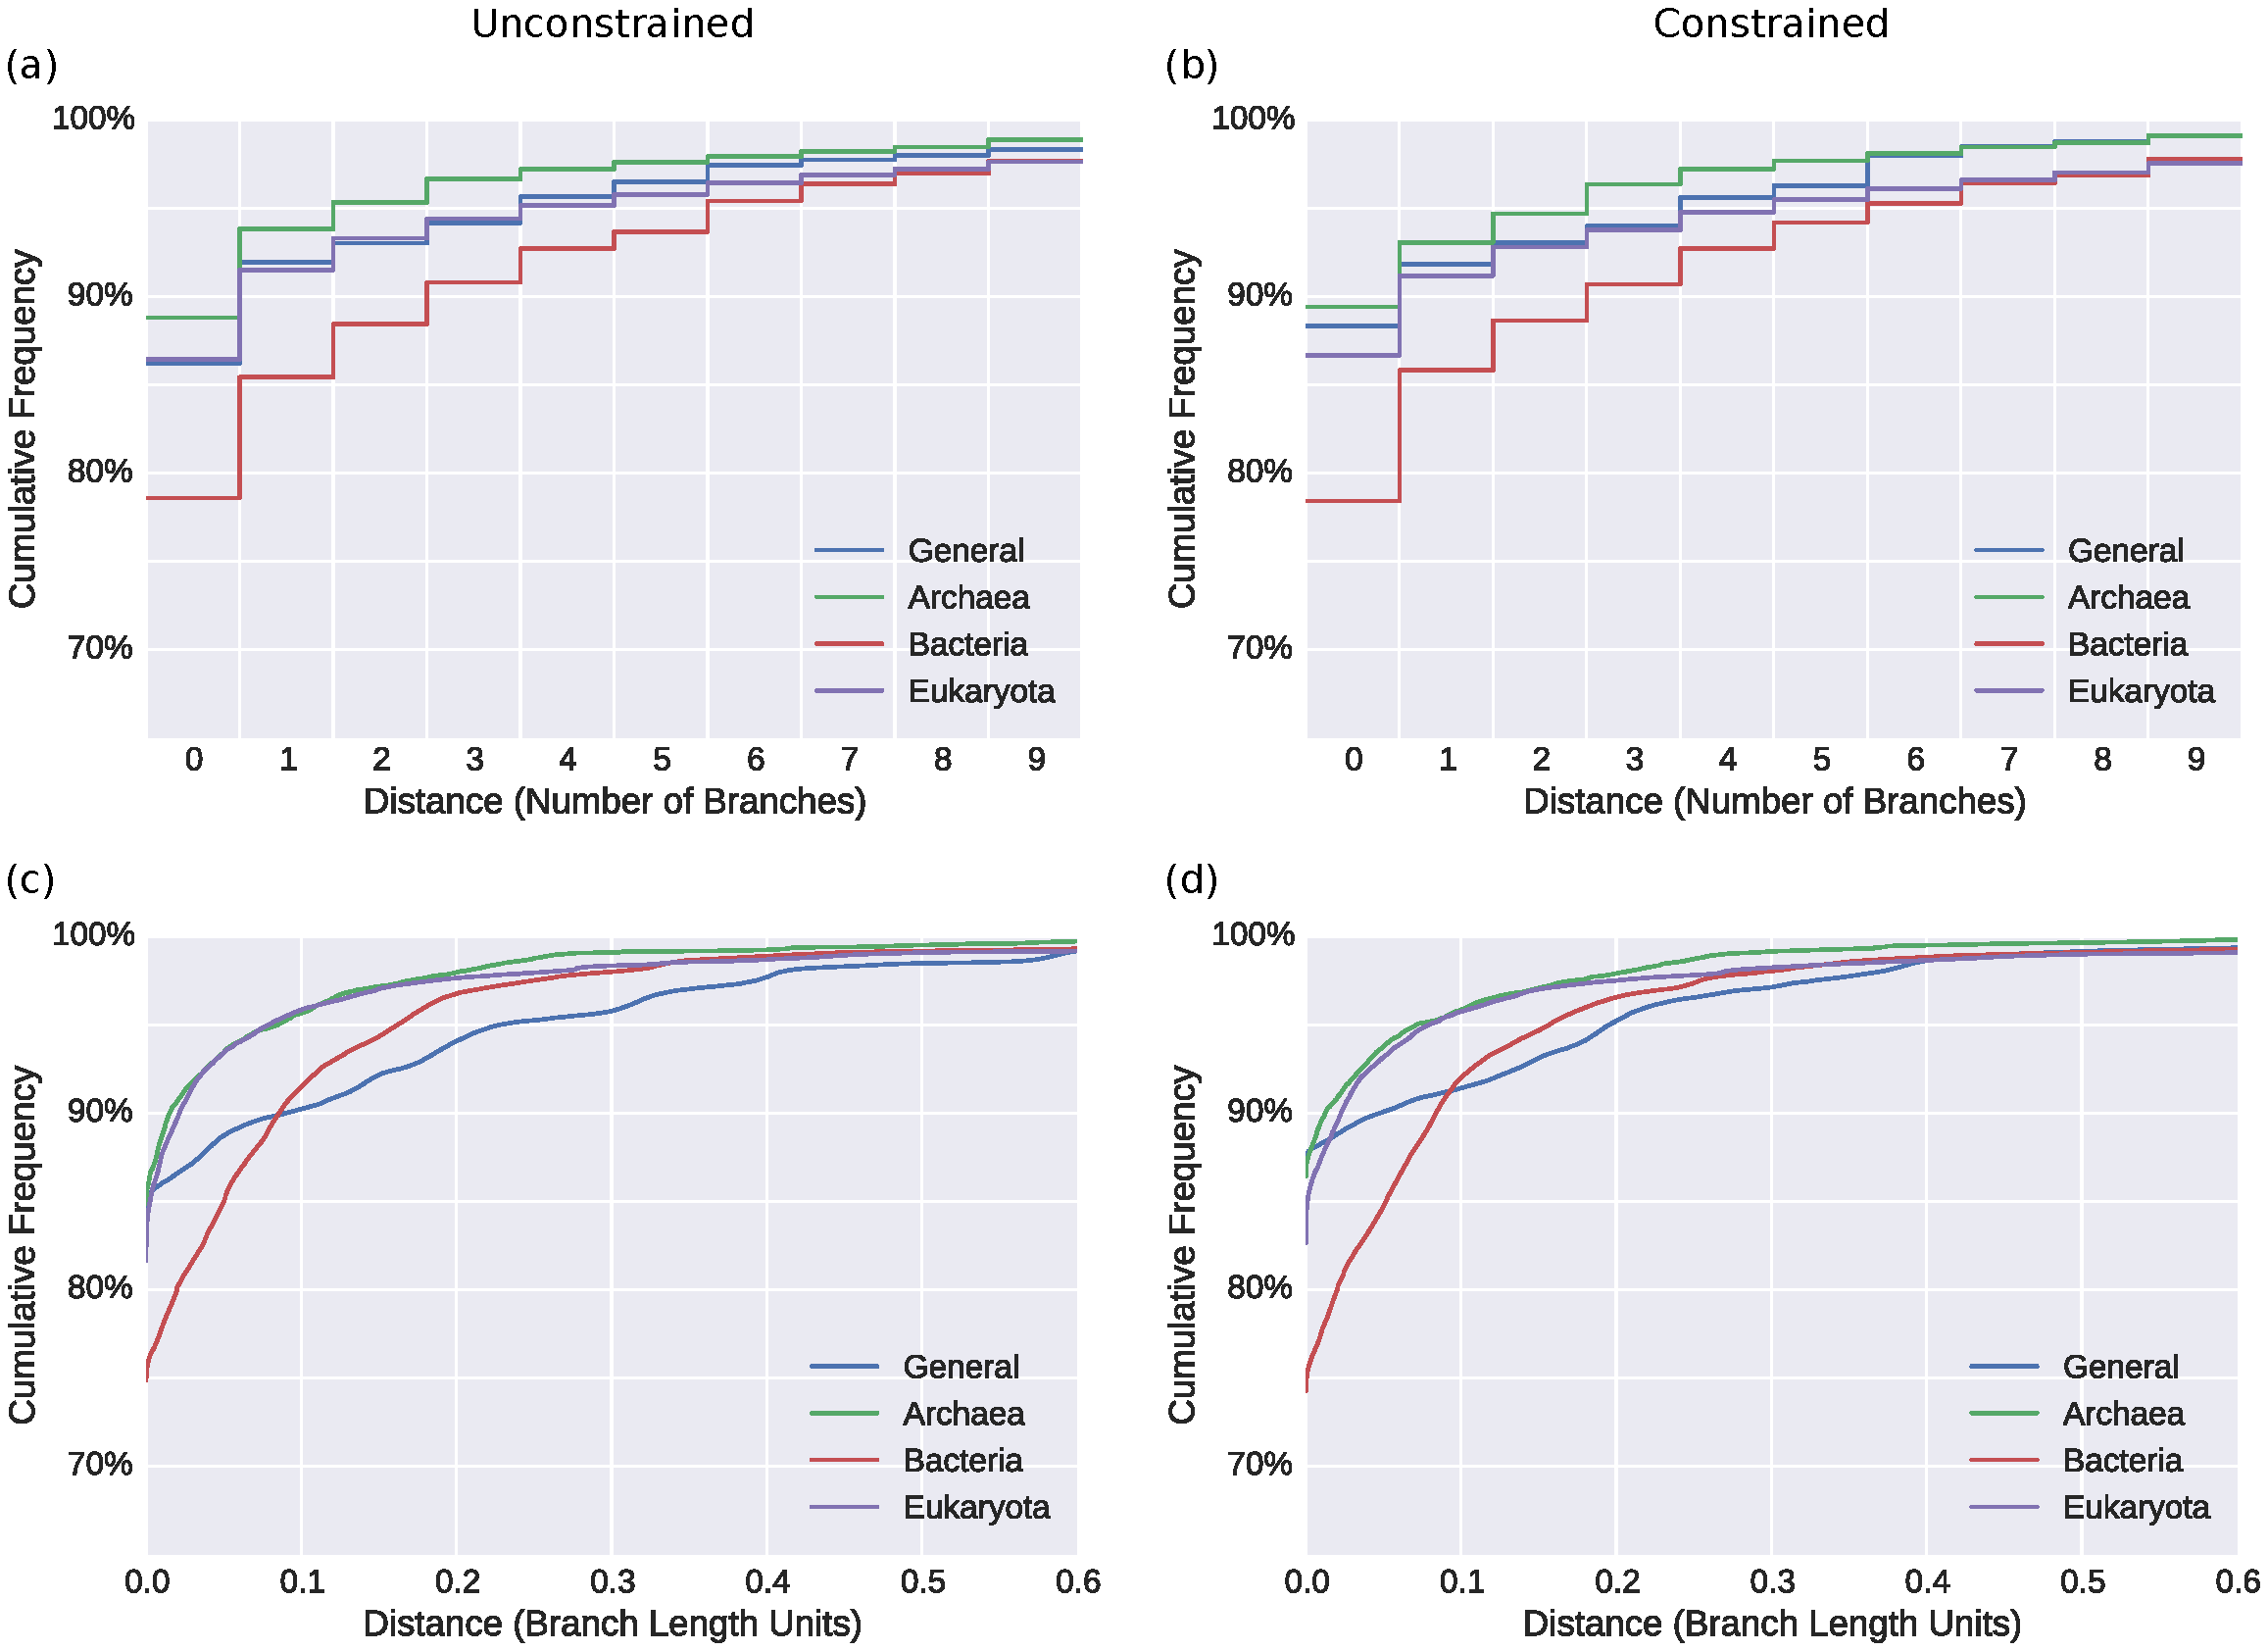
\includegraphics[width=\linewidth]{art/constraints_backbone.pdf}
    \begin{subfigure}{0pt}
        \phantomcaption
        \label{fig:constraints_backbone:sub:edge_unconstr}
    \end{subfigure}
    \begin{subfigure}{0pt}
        \phantomcaption
        \label{fig:constraints_backbone:sub:edge_constr}
    \end{subfigure}
    \begin{subfigure}{0pt}
        \phantomcaption
        \label{fig:constraints_backbone:sub:branch_unconstr}
    \end{subfigure}
    \begin{subfigure}{0pt}
        \phantomcaption
        \label{fig:constraints_backbone:sub:branch_constr}
    \end{subfigure}
%     Weighted distances to expected edges for
    \caption[Accuracy of the unconstrained and constrained \acsp{PhAT}]{
        \textbf{Accuracy of the unconstrained and constrained \acfp{PhAT}.}
        We evaluated the accuracy of our \acp{PhAT} by placing sequences
        and measuring the weighted distances to their respective expected placement branches.
        The figure shows the cumulative frequencies of number of sequences versus distances,
        measured in number of branches (top row, Subfigures \subref{fig:constraints_backbone:sub:edge_unconstr} and
        \subref{fig:constraints_backbone:sub:edge_constr})
        and in branch length units (bottom row, Subfigures \subref{fig:constraints_backbone:sub:branch_unconstr} and
        \subref{fig:constraints_backbone:sub:branch_constr}).
        In other words, it shows how many sequences are placed
        within a certain radius from their expected branches.
        For example, in \subref{fig:constraints_backbone:sub:edge_unconstr},
        more than 85\% of the sequences of the \taxonname{Bacteria} (red) are placed
        within a radius of at most one branch from their expected branch,
        and in \subref{fig:constraints_backbone:sub:branch_unconstr}, more than 95\% of the Eukaryota (purple) are
        within a radius of 0.1 branch length units from their expected branches.
        % If we for example want to know how accurately 80\% of the sequences were placed,
        % we follow the graph at 80\% down to the x-axis to find the wanted value.
        \\
        The figure compares the accuracy of using the unconstrained trees (left,
        Subfigures \subref{fig:constraints_backbone:sub:edge_unconstr} and \subref{fig:constraints_backbone:sub:branch_unconstr}) to
        using the \toolname{Silva} taxonomy as constraint for the tree inference (right, Subfigures
        \subref{fig:constraints_backbone:sub:edge_constr} and \subref{fig:constraints_backbone:sub:branch_constr}).
        As explained in \secref{ch:AutomaticTrees:sec:Evaluation:sub:ReferenceTreeSetup},
        the differences between the unconstrained and constrained trees mostly concern their inner branches,
        and thus are not expected to affect the accuracy much.
        This is confirmed by the fact that, overall, the results are similar between the pairs of trees.
        A slight improvement can be observed for the constrained General tree (blue),
        which performs better according to both distance measures.
        In most other cases, no significant differences can be observed.
%         Furthermore, the average branch length in all four constrained trees is longer
%         than in their respective unconstrained trees.
%         While this is in accordance with their lower likelihoods (see text),
%         this further helps in the placement process.
%         furthermore, the constr brings tips closer together, making their dist smaller,
%         in turn making the eval better for seqs that are close to those tips but not exact hits
    }
    \label{fig:constraints_backbone}
\end{figure}

% \begin{figure}[hpbt]
%     \centering
%     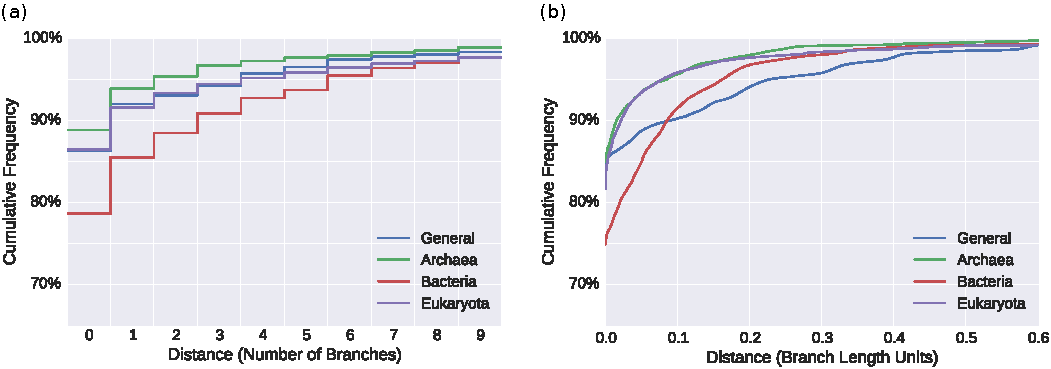
\includegraphics[width=\linewidth]{art/detail_majorities_backbone.pdf}
% %     \vspace*{-1em} %\todo{maybe not needed in the end}
%     \begin{subfigure}{0pt}
%         \phantomcaption
%         \label{fig:detail_majorities_backbone:sub:num_br}
%     \end{subfigure}
%     \begin{subfigure}{0pt}
%         \phantomcaption
%         \label{fig:detail_majorities_backbone:sub:br_dist}
%     \end{subfigure}
%     \caption[Weighted distances to expected edges for unconstrained trees]{
%         \textbf{Weighted distances to expected edges for unconstrained trees.}
%         We evaluated the accuracy of our \acp{PhAT} by placing sequences
%         and measuring the weighted distances to their respective expected placement branches.
%         The Figure shows the cumulative frequencies of number of sequences versus distances,
%         measured \subref{fig:detail_majorities_backbone:sub:num_br} in number of branches
%         and \subref{fig:detail_majorities_backbone:sub:br_dist} in branch length units.
%         In other words, it shows how many sequences are placed
%         within a certain radius from their expected branches.
%         For example, in \subref{fig:detail_majorities_backbone:sub:num_br},
%         more than 85\% of the sequences of the \taxonname{Bacteria} (red) are placed
%         within a radius of at most one branch from their expected branch,
%         and in \subref{fig:detail_majorities_backbone:sub:br_dist}, more than 95\% of the Eukaryota (purple) are
%         within a radius of 0.1 branch length units from their expected branches.
%     }
%     \label{fig:detail_majorities_backbone}
% %     \vspace*{-1em} %\todo{maybe not needed in the end}
% \end{figure}

% we are not using the continuous histogram plots any more. still, here are some notes that were meant for them:
% things are weighted by the lwr, so half edge dists can exist.
% explain why there are still jumps in the exact plots!
% (because of discrete number of placements per sequence!)
% accumulated percentage of number of placements within a radius of x edges of the correct placement location.
% the distance is weighted by lwrs, that is, the weighted average distance of each pquery is used,
% so that sub-edge resolution of the histogram is possible.

\afterpage{
\begin{landscape}
\begin{table}[htb]
\caption[Overview of the \acsp{PhAT} and their evaluation statistics]{
\textbf{Overview of the \acfp{PhAT} and their evaluation statistics.}
Details of four unconstrained (U) and four constrained (C) trees are shown.
``Size'' is the number of leaves of the tree, that is, the number of consensus sequences that the tree was inferred from,
see \tabref{tab:TreeTopologyTests}.
``\% Seqs.'' the percentage of sequences from \toolname{Silva} placed on it.
The \taxonname{General} tree does not cover all sequences,
because there are some sequence labels in the database that could not be mapped to the taxonomy.
``$\varnothing$ Br. Len.'' is the average branch length in the tree.
The evaluation results are reported in the remaining columns:
Average distances of the sequences to their respective expected branch are listed
in numbers of branches (Discrete) and in branch length units (Continuous), as explained in the text.
Furthermore, ``Exp. Br. Hits'' shows how often the most probable placement was placed exactly on the expected branch.
Lastly, the average expected distance between placement locations (EDPL) is shown.
The EDPL is the sum of the distances between the placements of a sequences weighted by their probability \citep{Matsen2010}.
}
\label{tab:ReferenceTreesOverview}
{
    \begin{center}
    \begin{tabular}{lrrrrrrr}
    \toprule
                                 &        &                &               & \multicolumn{2}{c}{Average Distance} &               &           \\
    Reference Tree               & Size   & \%\,Seqs.       & $\varnothing$\,Br.\,Len. & Discrete & Continuous       & Exp.\,Br.\,Hits & $\varnothing$\,EDPL \\
%     \hline
    \midrule
    \taxonname{General} (U)      &   1998 &    98.7\%      &         0.084 &          0.63 &                0.034 &     85.9\%    &   0.00058 \\
    \taxonname{General} (C)      &   1998 &    98.7\%      &         0.086 &          0.57 &                0.027 &     88.2\%    &   0.00046 \\
    \taxonname{Archaea} (U)      &    511 &     3.4\%      &         0.070 &          0.46 &                0.013 &     86.4\%    &   0.00038 \\
    \taxonname{Archaea} (C)      &    511 &     3.4\%      &         0.071 &          0.45 &                0.013 &     88.2\%    &   0.00041 \\
    \taxonname{Bacteria} (U)     &   1914 &    84.6\%      &         0.067 &          1.13 &                0.031 &     77.0\%    &   0.00095 \\
    \taxonname{Bacteria} (C)     &   1914 &    84.6\%      &         0.071 &          1.11 &                0.031 &     76.6\%    &   0.00091 \\
    \taxonname{Eukaryota} (U)    &   2059 &    10.0\%      &         0.080 &          0.79 &                0.022 &     84.9\%    &   0.00032 \\
    \taxonname{Eukaryota} (C)    &   2059 &    10.0\%      &         0.083 &          0.81 &                0.024 &     85.7\%    &   0.00031 \\
    \bottomrule
    \end{tabular}
    \end{center}
}
\end{table}
\end{landscape}
} %afterpage

% average branch lengths as mentioned above:
%
% constrained:
%
% arc  0.0717985
% bact 0.0709451
% euk  0.0830736
% gen  0.0859666
%
% avg  0.07794595
% min  0.0709451
% max  0.0859666
%
% unconstrained:
%
% arc  0.0697522
% bact 0.067082
% euk  0.0799271
% gen  0.084141
%
% avg  0.075225575
% min  0.067082
% max  0.084141

% On average, the distances in number of branches are between \num{0.46} (\taxonname{Archaea}) and \num{1.13} (\taxonname{Bacteria}),
% while the average distances in branch length units are between \num{0.014} (\taxonname{Archaea}) and \num{0.034} (\taxonname{General}).
% For comparison, the average branch lengths of the \acp{RT} are between \num{0.067} (\taxonname{Bacteria}) and \num{0.084} (\taxonname{General}).

Considering the size of the trees, most sequences are placed in close vicinity to their expected branches.
This is corroborated by the short average distances reported in \tabref{tab:ReferenceTreesOverview}.
Furthermore, the average expected distance between placement locations (EDPL) \cite{Matsen2010} is low,
indicating that the placements of a specific sequence mostly cluster in a small neighborhood of the tree.
We observed that errors occur mostly in parts of the tree with short branches,
which might be explained by the inability of 16S SSU sequences to properly resolve certain clades \citep{Janda2007}.
Also, the placement likelihood differences are small between neighboring, short branches,
such that the placement signal is fuzzy.

With 77\% of the sequences placed exactly on their expected branch,
the accuracy is generally lowest for the \taxonname{Bacteria} tree.
This might be because the \taxonname{Bacteria} have the most sequences in \toolname{Silva}, and exhibit a high diversity.
In the other three trees, more than 90\% of the sequences are placed
at most one branch away from their respective expected branch.
The constrained trees exhibit similar placement accuracy,
indicating that the differences in the inner branches of the trees indeed do not substantially affect the placement accuracy.
Finally, we note that the results are reported without any manual corrections, and use overly broad \acp{RT}.
Thus, in real world studies, where trees are often more specific for a clade of interest,
better results are to be expected.
Particularly when using Multilevel Placement with overlapping \acp{RT},
placement differences of a few branches on the first level tree are acceptable,
as they do not change the second level tree on which the sequence is placed;
see \secref{ch:AutomaticTrees:sec:Evaluation:sub:MultilevelPlacement} for details.

\paragraph{Different Consensus Methods}
\label{ch:AutomaticTrees:sec:Evaluation:sub:Accuracy:par:ConsensusMethods}

As outlined in the method description (see \secref{ch:AutomaticTrees:sec:Methods:sub:PhAT:par:SequenceGrouping}),
we represent clade diversity via majority rule consensus sequences.
To assess the impact of the consensus method on the placement accuracy,
we repeated the above evaluation using alternative consensus methods.
In particular, we used Cavener's method \citep{Cavener1987,Cavener1991a},
and threshold consensus sequences \citep{Day1992a,Day1992}.
As shown in \figref{fig:consensi_backbone}, we found little difference between the methods.

\begin{figure}[hpbt]
    \centering
    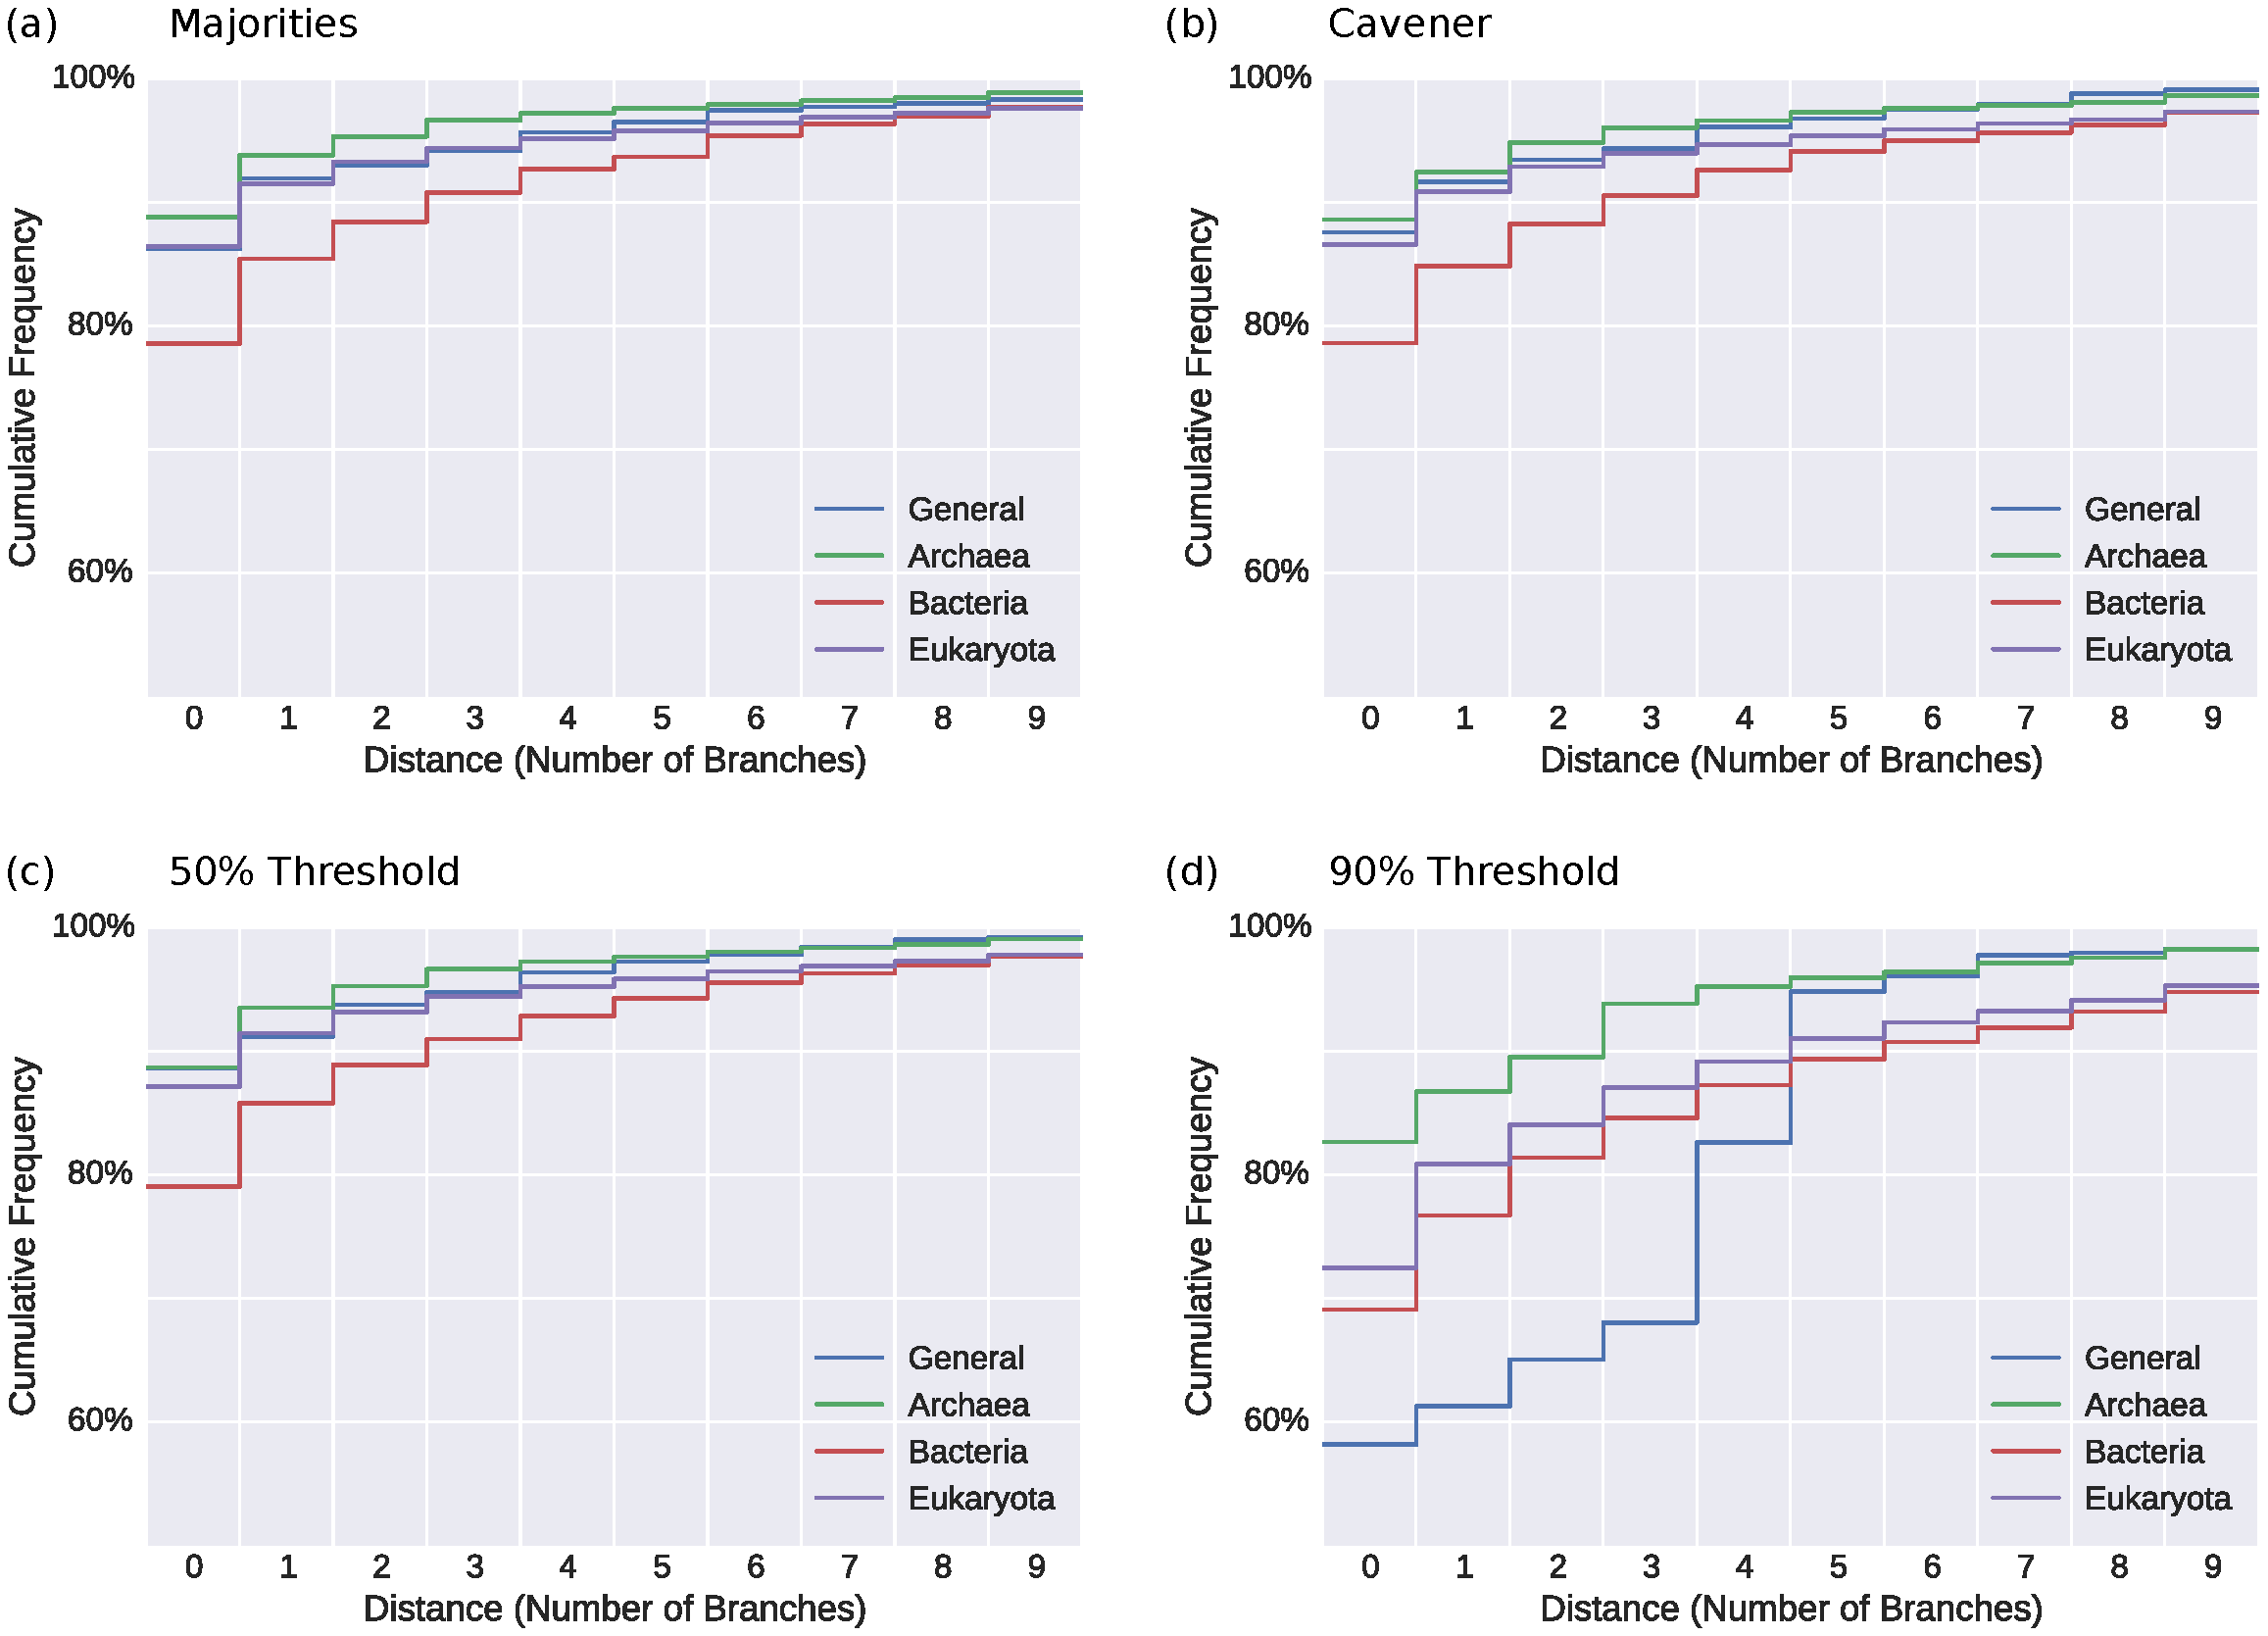
\includegraphics[width=\linewidth]{art/consensi_backbone.pdf}
    \begin{subfigure}{0pt}
        \phantomcaption
        \label{fig:consensi_backbone:sub:majorities}
    \end{subfigure}
    \begin{subfigure}{0pt}
        \phantomcaption
        \label{fig:consensi_backbone:sub:cavener}
    \end{subfigure}
    \begin{subfigure}{0pt}
        \phantomcaption
        \label{fig:consensi_backbone:sub:50_threshold}
    \end{subfigure}
%     \begin{subfigure}{0pt}
%         \phantomcaption
%         \label{fig:consensi_backbone:sub:70_threshold}
%     \end{subfigure}
    \begin{subfigure}{0pt}
        \phantomcaption
        \label{fig:consensi_backbone:sub:90_threshold}
    \end{subfigure}
%     \begin{subfigure}{0pt}
%         \phantomcaption
%         \label{fig:consensi_backbone:sub:95_threshold}
%     \end{subfigure}
    \caption[Effect of different consensus sequence methods on accuracy]{
        \textbf{Effect of different consensus sequence methods on accuracy.}
        In the main evaluation of our \ac{PhAT} method,
        we use reference trees and alignments based on majority rule consensus sequences \citep{May1952,Day1992a}
        of the \toolname{Silva} database sequences.
        Here, we evaluate the effect of using other consensus sequence methods
        on phylogenetic placement accuracy.
%         The evaluation method is described in the text.
        In addition to \subref{fig:consensi_backbone:sub:majorities} majority rule consensus, we tested
        \subref{fig:consensi_backbone:sub:cavener} Cavener's method \citep{Cavener1987,Cavener1991a},
        as well as threshold consensus sequences \citep{Day1992a,Day1992}
        using thresholds of 50\%, 60\%, 70\%, 80\%, and 90\%, of which two are shown in
        \subref{fig:consensi_backbone:sub:50_threshold} and \subref{fig:consensi_backbone:sub:90_threshold}.
        The three remaining threshold methods exhibit accuracies almost exactly in between the shown plots,
        that is, accuracy decreases with increasing thresholds.
%         and thus are excluded here for simplicity.
        For comparison, we also included \figref{fig:constraints_backbone:sub:edge_unconstr} again,
        here as Subfigure~\subref{fig:consensi_backbone:sub:majorities},
        using the same y-axis scaling as the other plots.
        All trees used in this part of the evaluation are unconstrained.
        We only show distances measured in number of branches here,
        because this is more relevant in the context of our methods.
        % for evaluating phylogenetic placement.
    }
    \label{fig:consensi_backbone}
\end{figure}

By using alternative consensus methods, the consensus sequences and thus the sites in the alignments change.
Furthermore, we used random initial starting trees for the tree inference.
Hence, the obtained reference trees (not shown) differ substantially from each other.
Across the corresponding trees of the tested consensus methods,
we observed an average relative Robinson-Foulds distance \citep{Robinson1981}
(see \secref{ch:Foundations:sec:TreeOfLife:sub:PhylogeneticTrees:par:TreeProperties}) of 49.5\%.
This is similar to our findings depicted above, e.g., in \figref{fig:constraints_backbone}.
For the different consensus methods, again,
the accuracy of their respective constrained variants of these trees (data not shown)
does not change much compared to the accuracy obtained for the unconstrained trees shown in \figref{fig:consensi_backbone}.
Thus, the differences in accuracy seen in the Figure are most likely due to
the interplay of alignment and placed sequences (which is what we are interested in),
and not due to differences in the trees (which are not of interest here).

The first three plots in \figref{fig:consensi_backbone:sub:majorities}--\subref{fig:consensi_backbone:sub:50_threshold}
exhibit similar accuracies.
On average, majority rule, Cavener's, and low threshold ($\leq$ 70\%) consensus methods
place 82--83\% of the sequences on the expected branch.
As a general trend, the \taxonname{Archaea}, being the smallest tree, tend to have the highest accuracy.
On the other hand, the \taxonname{Bacteria}, having the most sequences in \toolname{Silva}, score worst.
This changes for high consensus thresholds. %, e.g., \figref{fig:consensi_backbone:sub:90_threshold}.
At high thresholds, many sites contain ambiguity characters, thus blurring the phylogenetic signal.
The \taxonname{General} tree, representing the highest diversity, is most affected by this,
as can be seen in the last two plots \figref{fig:consensi_backbone:sub:50_threshold}
and \figref{fig:consensi_backbone:sub:90_threshold}.

\paragraph{Actual Sequences}
\label{ch:AutomaticTrees:sec:Evaluation:sub:Accuracy:par:SingleSequences}

For the above evaluations of the \ac{PhAT} method,
we used some form of consensus sequence representation for the clades of the taxonomy,
see e.g., \figref{fig:constraints_backbone} and \figref{fig:consensi_backbone}.
However, we also tested how the method behaves when using actual sequences from the database instead
to represent the taxonomic clades,
thus avoiding to unnecessarily blur the phylogenetic signal,
and other potential drawback of consensus sequences.

As manually selecting representative sequences from the database was not practical,
we used the following automated approach.
First, we took the 90\% threshold consensus sequences of the \ac{PhAT} method
that were already evaluated in \figref{fig:consensi_backbone:sub:90_threshold}.
By using a high threshold, most of the diversity of each clade is included.
Then, for each such consensus sequence,
we calculated a score for all sequences from the database that were used to construct this consensus sequence.
This score is the number of different nucleotides between the consensus sequence and the database sequence.
The sequence with the lowest score (that is, with most matching nucleotides)
was then used as representative of the clade.
Thereby, the taxonomic clades are represented by actual sequences from the database.
However, as these sequences are close to the respective consensus sequence,
they are still good representatives of the diversity of the clade.
%         They can hence be considered to be good representatives of the clades.
This resulted in a set of sequences of the same size as the original set of consensus sequences.
Using these sequences, we then again inferred a tree and
conducted the evaluation procedure by placing all sequences of the database on that tree,
as described before.
The results for the four unconstrained trees is shown in \figref{fig:single_seqs}.

\begin{figure}[hpbt]
    \centering
    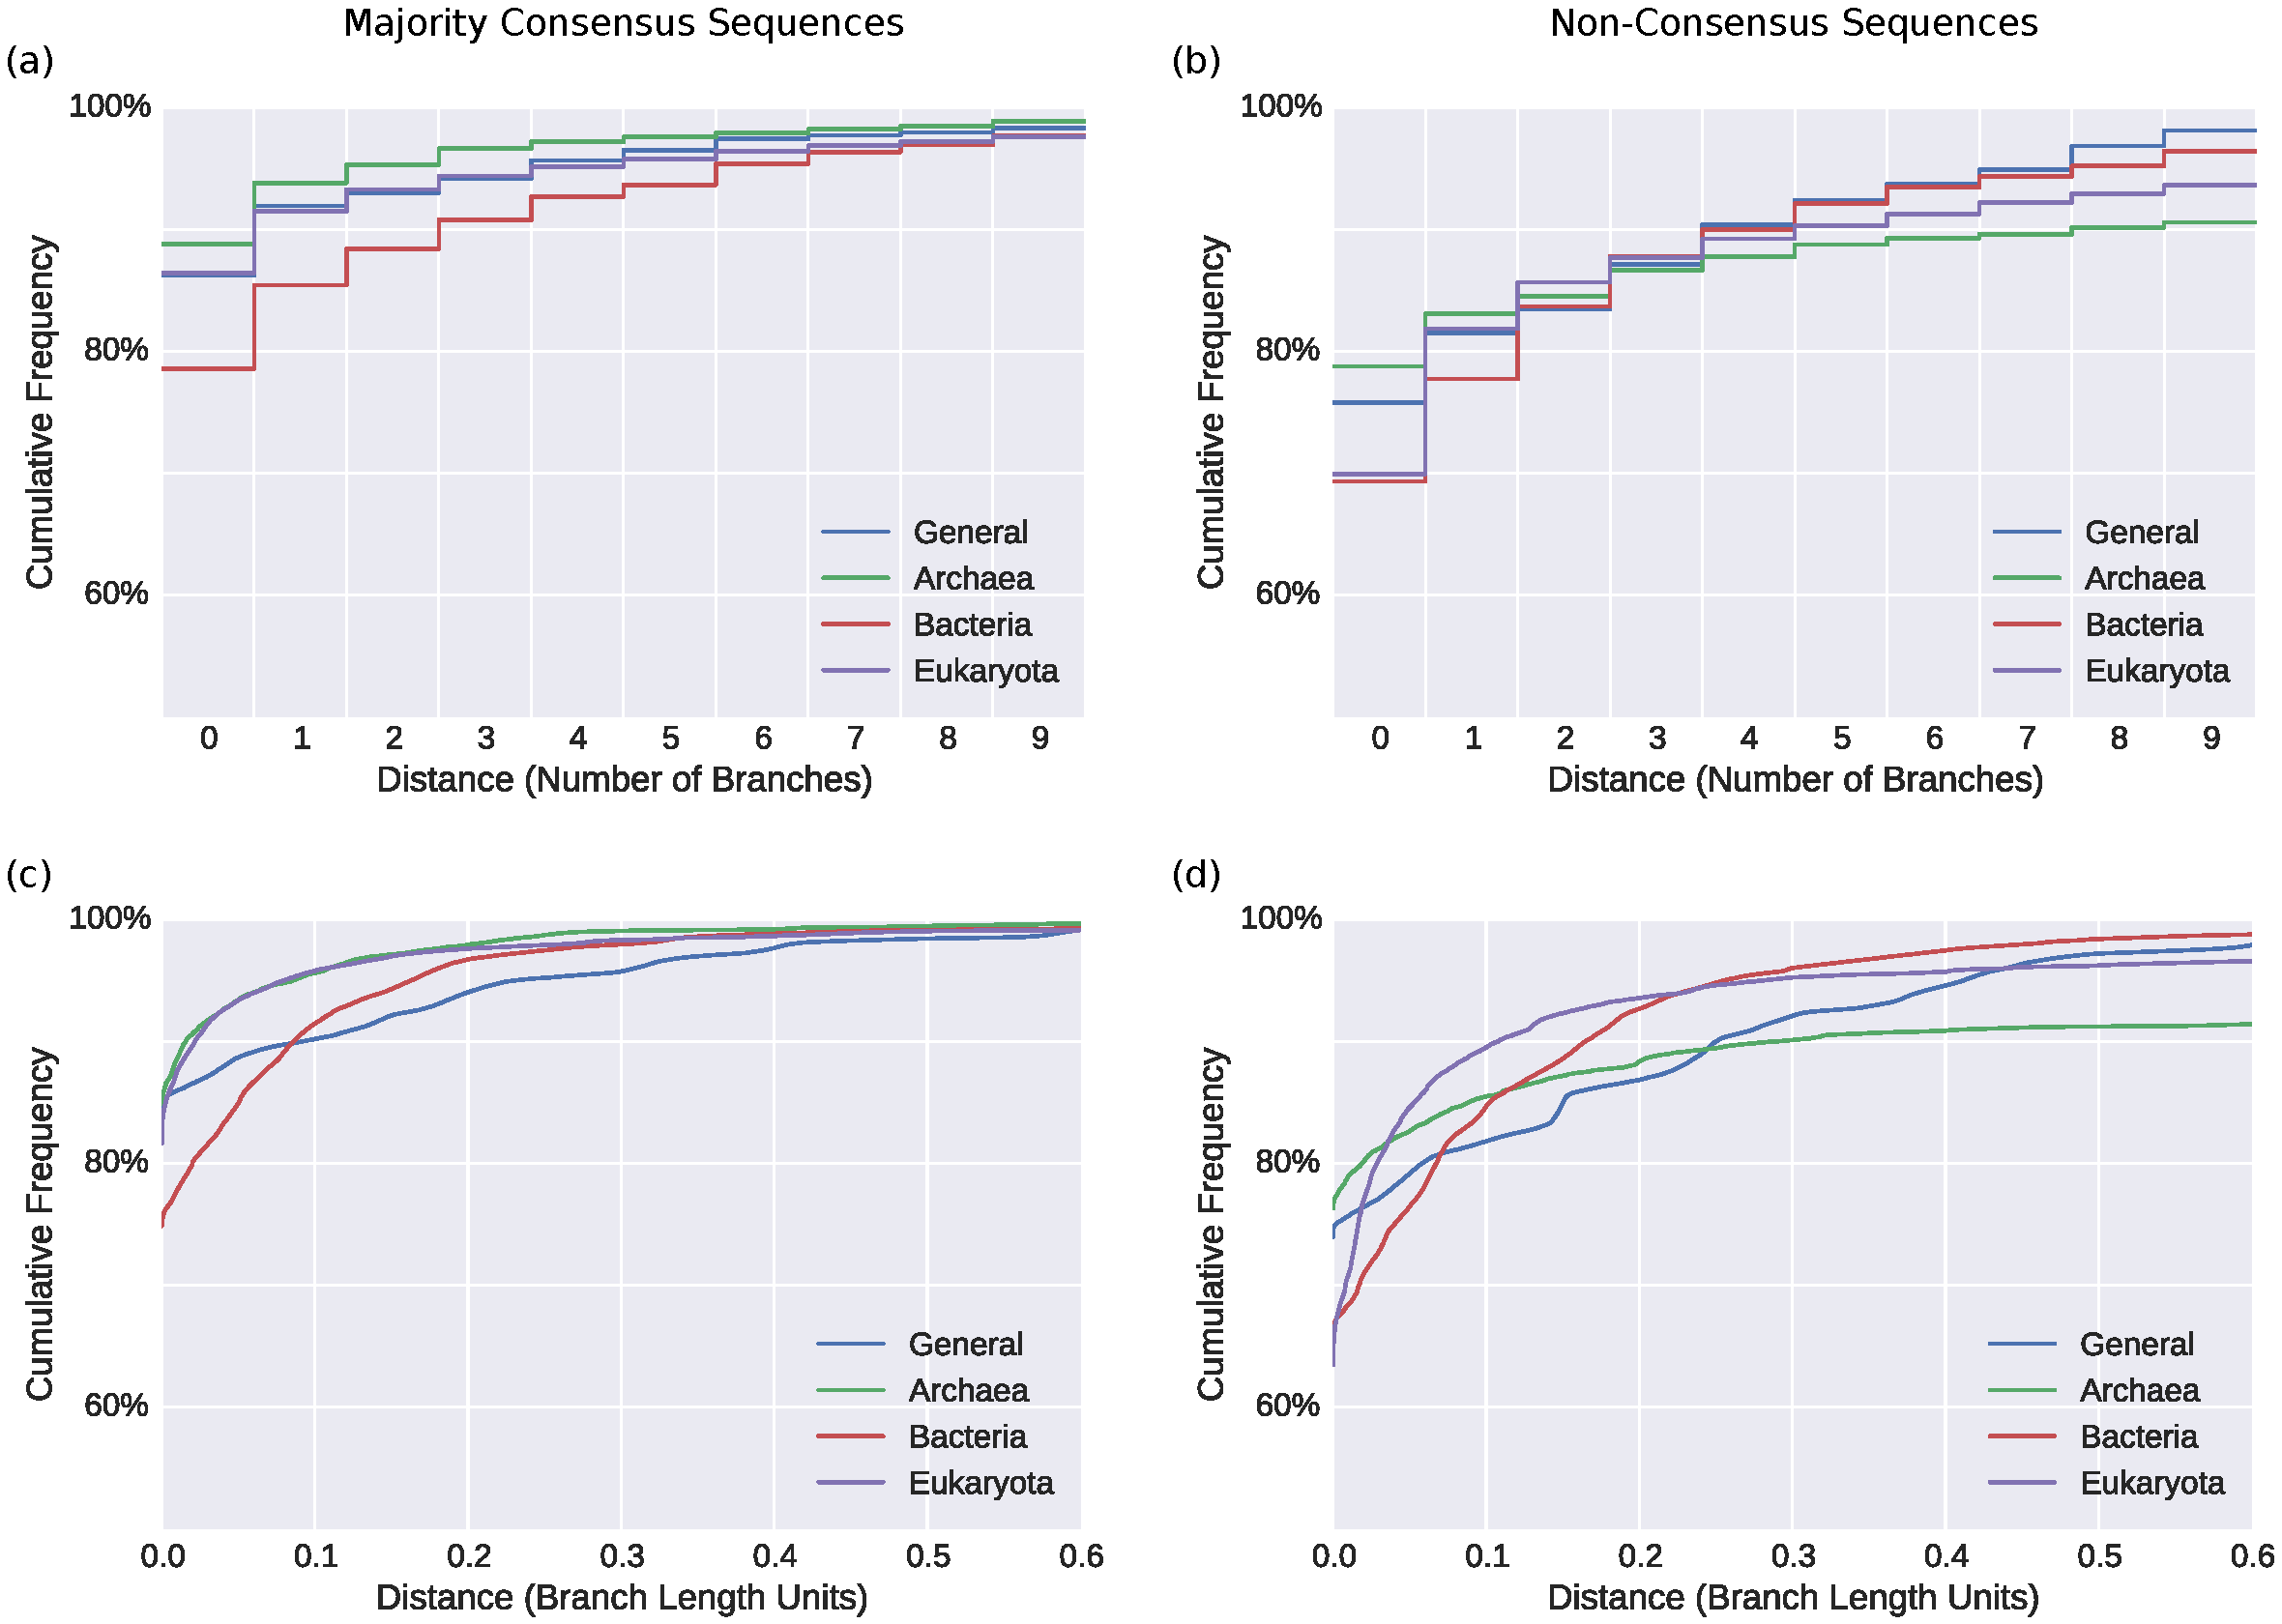
\includegraphics[width=\linewidth]{art/single_seqs.pdf}
    \begin{subfigure}{0pt}
        \phantomcaption
        \label{fig:single_seqs:sub:majorities_edge}
    \end{subfigure}
    \begin{subfigure}{0pt}
        \phantomcaption
        \label{fig:single_seqs:sub:single_seq_edge}
    \end{subfigure}
    \begin{subfigure}{0pt}
        \phantomcaption
        \label{fig:single_seqs:sub:majorities_branch}
    \end{subfigure}
    \begin{subfigure}{0pt}
        \phantomcaption
        \label{fig:single_seqs:sub:single_seq_branch}
    \end{subfigure}
    \caption[Effect of using actual sequences on placement accuracy]{
        \textbf{Effect of using actual sequences (instead of consensus sequences) on placement accuracy.}
        Subfigures~\subref{fig:single_seqs:sub:majorities_edge}
        and \subref{fig:single_seqs:sub:majorities_branch}
        show the evaluation of the majority rule consensus sequences, and are identical to
        \figref{fig:constraints_backbone:sub:edge_unconstr} and \figref{fig:constraints_backbone:sub:branch_unconstr},
        respectively.
        They are included here for ease of comparison, however with the y-axis scaled to fit the remaining subfigures.
        Subfigures~\subref{fig:single_seqs:sub:single_seq_edge} and \subref{fig:single_seqs:sub:single_seq_branch}
        show the evaluation of the approach of using actual sequences from the database (instead of consensus sequences),
        as explained in the text.
        The top row (Subfigures \subref{fig:single_seqs:sub:majorities_edge} and \subref{fig:single_seqs:sub:single_seq_edge})
        shows distances in number of branches away from the expected placement branch;
        the bottom row (Subfigures \subref{fig:single_seqs:sub:majorities_branch} and \subref{fig:single_seqs:sub:single_seq_branch})
        shows distances in branch length units.
        All trees used for this evaluation are unconstrained.
    }
    \label{fig:single_seqs}
\end{figure}

We found that this approach yields trees that are less accurate for phylogenetic placement.
The resulting accuracy is worse in all cases.
That is, on average, the sequences were placed further from their respective expected branch.
We suspect that this is (i) because single sequences do not capture the diversity of their clade
as well as consensus sequences,
and (ii) because they do not incorporate as much biological information (e.g., in form of ambiguity characters).
We hence conclude that using consensus sequences to represent clades in our \ac{PhAT} approach is superior.

\paragraph{Further Aspects and Observations}
\label{ch:AutomaticTrees:sec:Evaluation:sub:Accuracy:par:FurtherAspectsAndObservations}

In the evaluations above, we generally found that using a constraint
when inferring the tree only slightly changes the accuracy of our evaluation.
However, when considering only the distance of the most likely placement (highest \ac{LWR}) to its correct edge
instead of using average distances weighted by the \ac{LWR} per \ac{QS},
the constrained trees consistently yield better results (data not shown).
In other words, the most likely placement is more often on the correct branch of the constrained trees.
For example, the most significant change is observed for the Eukaryota tree,
with 84\% correct placements for the unconstrained tree, but 89\% for the constrained one.
We suspect that this is an artifact of our evaluation process,
as we consider a sequence to be correctly placed if the placement branch belongs to the consensus sequence
to which the sequence contributed.
As the selection of sequences for each consensus sequence is guided by the taxonomy,
using the same taxonomy as constraint for the tree thus might also improve the placement accuracy.

As a final remark, we implicitly assumed the taxonomic label of each sequence to be correct.
That is, in the evaluations, we measured the accuracy of the placements
using the taxonomic labels of the sequences in \toolname{Silva} as an indicator of the expected branch of each sequence.
However, errors are expected due to incongruity between the taxonomy and the phylogeny \citep{Moreira2000},
as well as due to taxonomically mislabeled sequences \citep{Kozlov2016}.
For example, \toolname{Sativa} \citep{Kozlov2016},
% which evaluated the same version of the \toolname{Silva} database that we used,
found \num{9 934} mislabeled sequences in the \toolname{Silva} database.
Furthermore, \num{17 452} sequences contain one of ``incertae'', ``unclassified'' or ``unknown'' in their name,
indicating that those sequences might not be reliable.
In total, there are \num{25 910} (or \num{4.3}\%) such dubious sequences in version 123.1 of the \toolname{Silva} database.
Not all sequences are hence expected to be placed on their expected branches.
% sativa mislabels   9 934
% incertae          12 002
% unknown            5 446
% unclassified           4
% total blacklist   25 910
% total sequences  598 470
We thus evaluated how these dubious sequences affect the accuracy of the trees.
To this end, we used the same four trees as used in the main part of the evaluation
(that is, they were constructed with all sequences, including the dubious sequences),
but for the evaluation step itself excluded the dubious sequences.
That is, those sequences were not placed on the trees,
and their distance to the expected branch was not used for the evaluation.
In most cases, this improved the results slightly, but not by much (data not shown).
This shows that our trees are also robust to such uncertain sequences.
Therefore, we decided to only report the unfiltered results in the above evaluations.

% Thus, we have to assume the taxonomic label of each sequence to be correct.
% However, errors are expected due to incongruence between the taxonomy and the phylogeny \citep{Moreira2000},
% as well as due to taxonomically mislabeled sequences \citep{Kozlov2016}.
% Furthermore, sequences containing ``incertae'', ``unclassified'' or ``unknown'' in their name
% indicate that those sequences might not be reliable.
% In total, there are \num{25 910} (or \num{4.3}\%) such dubious sequences in version 123.1 of the \toolname{Silva} database.
% Not all sequences are hence expected to be placed on their expected branches.
% We also ran the evaluation with those sequences excluded,
% which in most cases improved the results slightly (data not shown),
% but report the unfiltered results here.

% ======================================================================================================================
%     Empirical Datasets
% ======================================================================================================================

\subsection{Empirical Datasets}
\label{ch:AutomaticTrees:sec:Evaluationsub:EmpiricalDatasets}

\acp{PhAT} are intended for conducting phylogenetic placement of environmental sequences.
As the true evolutionary history of such sequences is unknown,
we can not repeat the previous accuracy tests on empirical environmental datasets.
Instead, we assess if the \acp{PhAT} yield meaningful quantitative results for typical post-analysis methods.
To this end, we placed two empirical metagenomic amplicon barcoding datasets on our unconstrained \taxonname{Bacteria} tree.
To asses the placement results obtained from the \ac{PhAT},
we performed Squash Clustering and Edge PCA \citep{Matsen2011a} post-analyses on the placement results
(see \secref{ch:EmpiricalDatasets} and
\figref{fig:bv_squash}, \figref{fig:bv_edgepca} and \figref{fig:hmp_mds_epca} for details).
The results reveal that the \ac{PhAT} reproduces results of previous studies
based on custom \acp{RT} with manually selected reference sequences.
Furthermore, the \ac{PhAT} is able to classify samples (e.g., healthy vs sick patients),
at least to the extend that is expected from its phylogenetic resolution.
That is, samples that only differ in placements at the species level
cannot be classified using a broad, high-level tree such as our \taxonname{Bacteria} tree.
In order to obtain finer taxonomic resolution, it is thus necessary to either use a \ac{PhAT} that contains more taxa,
or to use our multilevel approach instead (see next Section).


Here, we test the behavior of the unconstrained \taxonname{Bacteria} tree obtained via our \ac{PhAT} method
when used for standard post-analyses of phylogenetic placement results.
For this, we used a sequence dataset of the vaginal microbiome of 220 women \citep{Srinivasan2012}.
For details on the processing, see \secref{ch:EmpiricalDatasets}.
% containing a total of \num{426 612} sequences.
The original study showed associations between the presence of certain bacterial species
and the diagnosis of \acf{BV}, a condition caused by changes in the vaginal microbiome.
In the study, the Nugent score \citep{Nugent1991} was used as a clinical diagnostic criterion for \ac{BV},
which ranges from \num{0} (healthy) to \num{10} (severe illness).
We placed the sequences of the dataset on their original tree and on our \ac{PhAT},
and reproduce some of the results from the original study
% by performing Squash Clustering and Edge PCA on the data
to assess differences induced by using distinct references trees.
% Each colored dot in the figure represents one sample.

%         moved to intro:
        Squash Clustering is a hierarchical clustering method for phylogenetic placement data \citep{Matsen2011a} % and Srinivasan2012
%         It is a generalization of the UniFrac distance \citep{Lozupone2005,Lozupone2007a},
%         and yields meaningful branch lengths of the cluster tree.
%         To this end, it
        that uses the phylogenetic Kantorovich-Rubinstein (KR) distance \citep{Evans2012} % and Matsen2011a
%         also known as the Wasserstein distance, Mallows distance,
%         or Earth Mover's distance \citep{Mallows1972,Rachev1985,Levina2001,Villani2008},
        to measure cluster similarity.
        The result of Squash Clustering is a cluster tree of samples,
        where samples that are similar according to the KR distance are closer to each other,
        with branch lengths according to that distance.



The general features of the two cluster trees are comparable,
indicating that our tree is able to distinguish between healthy and sick patients.
However, there is a major difference in the lower half of the trees:
While \subref{fig:bv_squash:sub:squash_orig} shows some small branch lengths and even a separated sub-clade
of samples with low Nugent score,
these branches have a length of virtually zero in \subref{fig:bv_squash:sub:squash_art}.
As shown in \citep{Srinivasan2012}, the healthy patients are divided into two classes,
based on the presence of two species of \taxonname{Lactobacillus}.
The original reference tree contains sequences of those species, and can thus distinguish between them.
Our broad \taxonname{Bacteria} tree however
does not have this degree of species-level resolution and thus treats them the same,
yielding a negligible KR distance between the samples.
Although this finding is expected, it serves as an example for the limits of our method.

    moved to intro:
    Edge PCA \citep{Matsen2011a} is a dimensionality reduction method for phylogenetic placement data,
    which can visualize differences between samples.
       ---

While our tree is able to separate samples by Nugent score,
it does not exhibit the further separation of the two \taxonname{Lactobacillus} species
that is apparent when using the original tree.
Thus, the samples with low Nugent score form one blob in \figref{fig:bv_edgepca:sub:edgepca_art}.

This limitation can be overcome by either resolving the \ac{PhAT} down to species level,
or by using multilevel placement with a refined tree
that for example contains species sequences of the relevant \taxonname{Lactobacillus} clades.
We however generally note that similar issues of deficient resolution or missing species
can potentially also arise when hand-selecting reference sequences.
In the end, it is the responsibility of the researcher to make sure that the selection of reference sequences
is suitable for the dataset to be placed.

\begin{figure}[hpbt]
    \centering
    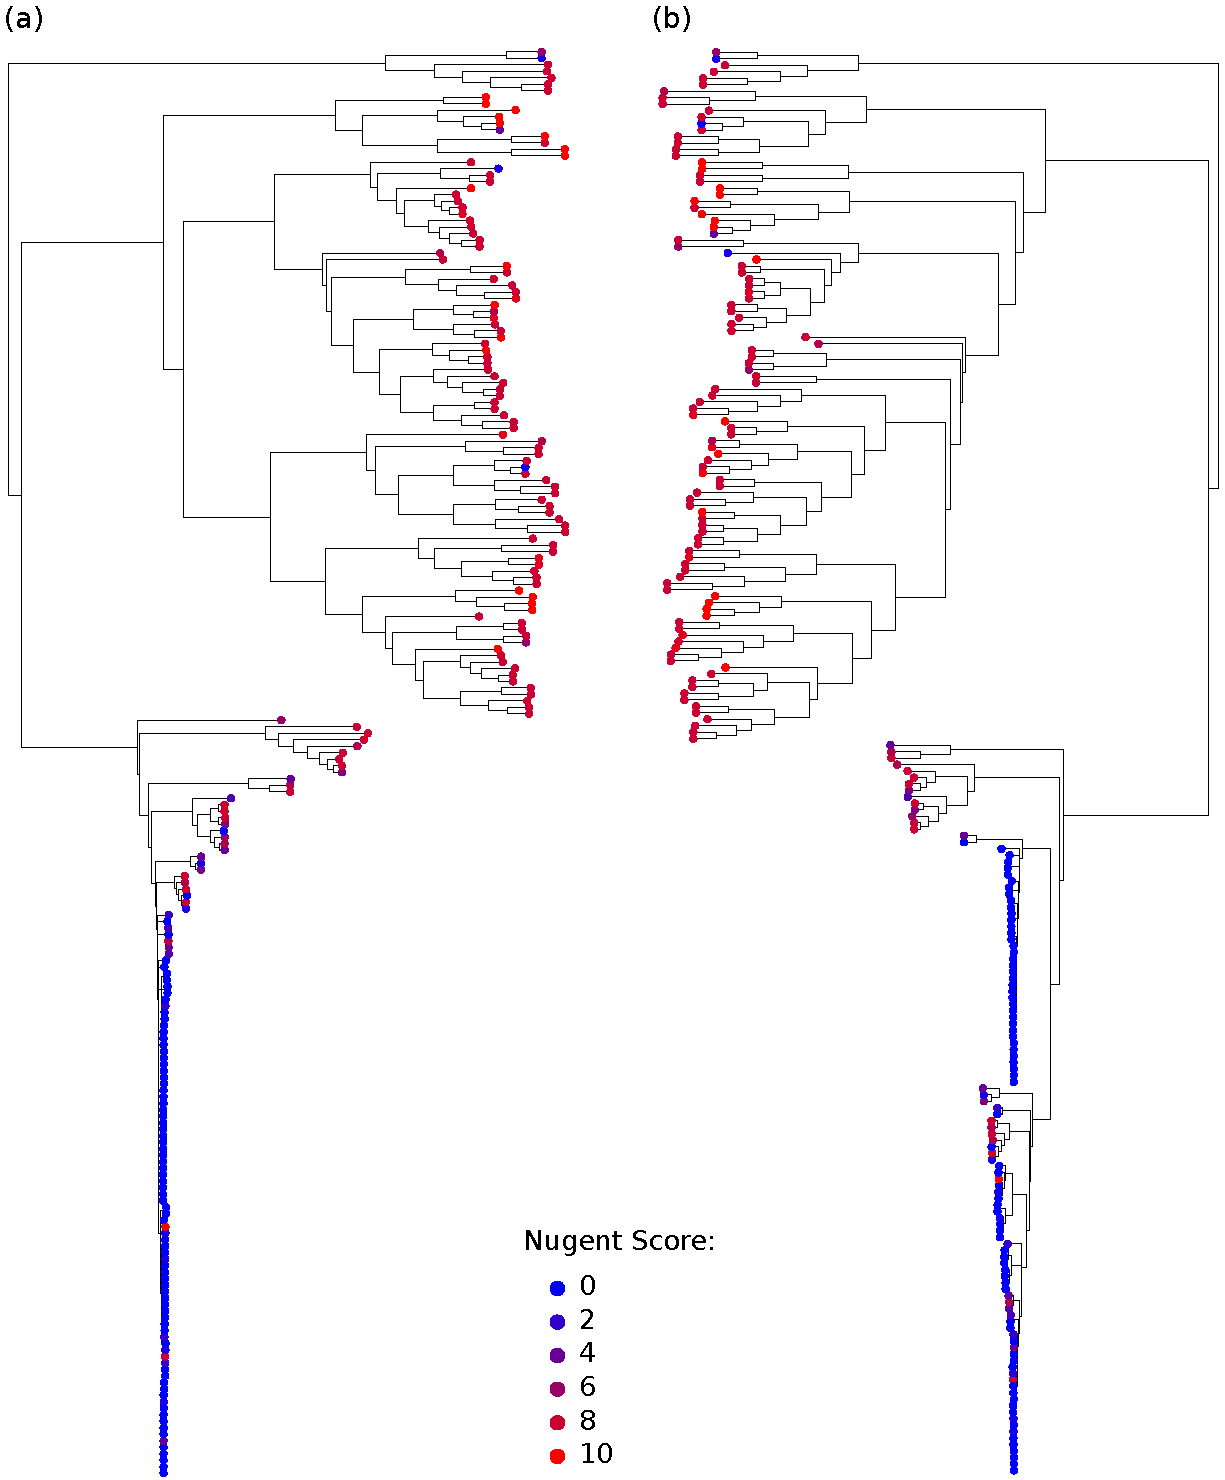
\includegraphics[width=\linewidth]{bv_squash.pdf}
    \begin{subfigure}{0pt}
        \phantomcaption
        \label{fig:bv_squash:sub:squash_art}
    \end{subfigure}
    \begin{subfigure}{0pt}
        \phantomcaption
        \label{fig:bv_squash:sub:squash_orig}
    \end{subfigure}
    \caption[Assessment of a \acs{PhAT} for conducting Squash Clustering]{
        \textbf{Assessment of a \acs{PhAT} for conducting Squash Clustering.}
        The Figure compares the hierarchical clustering trees resulting from a Squash Clustering analysis
        (see \secref{ch:Foundations:sec:PhylogeneticPlacement:sub:ExistingMethods:par:SquashClustering})
        using \subref{fig:bv_squash:sub:squash_art}  our unconstrained \taxonname{Bacteria} \acs{PhAT} and
        \subref{fig:bv_squash:sub:squash_orig} the original reference tree of \citep{Srinivasan2012}.
        Subfigure \subref{fig:bv_squash:sub:squash_orig} is a recalculation of Figure~1(A) of \citep{Srinivasan2012},
        and horizontally flipped for ease of comparison.
        The tips of both clustering trees correspond to samples,
        which are colored by the respective Nugent score of each sample,
        where higher values indicate women with severe \acl{BV}.
    }
    \label{fig:bv_squash}
\end{figure}

\begin{figure}[hpbt]
    \centering
    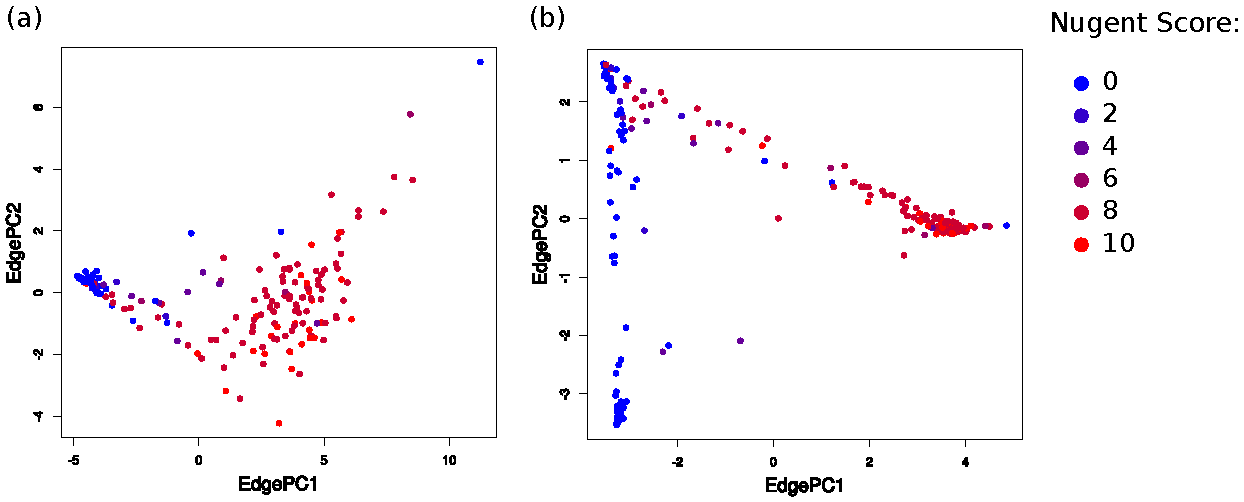
\includegraphics[width=\linewidth]{bv_edgepca.pdf}
    \begin{subfigure}{0pt}
        \phantomcaption
        \label{fig:bv_edgepca:sub:edgepca_art}
    \end{subfigure}
    \begin{subfigure}{0pt}
        \phantomcaption
        \label{fig:bv_edgepca:sub:edgepca_orig}
    \end{subfigure}
    \caption[Assessment of a \acs{PhAT} for conducting Edge PCA]{
        \textbf{Assessment of a \acs{PhAT} for conducting Edge PCA.}
        The Figure compares the scatter plots resulting from an Edge PCA
        (see \secref{ch:Foundations:sec:PhylogeneticPlacement:sub:ExistingMethods:par:EdgePCA})
        using \subref{fig:bv_edgepca:sub:edgepca_art} our unconstrained \taxonname{Bacteria} \acs{PhAT} and
        \subref{fig:bv_edgepca:sub:edgepca_orig} the original reference tree of \citep{Srinivasan2012}.
        Subfigure \subref{fig:bv_edgepca:sub:edgepca_orig} is a recalculation of Figure~3(A) of \citep{Srinivasan2012}.
        The items represent samples, which are colored by the respective Nugent score of each sample,
        where higher values indicate women with severe \acl{BV}.
    }
    \label{fig:bv_edgepca}
\end{figure}

\begin{figure}[hpbt]
    \centering
    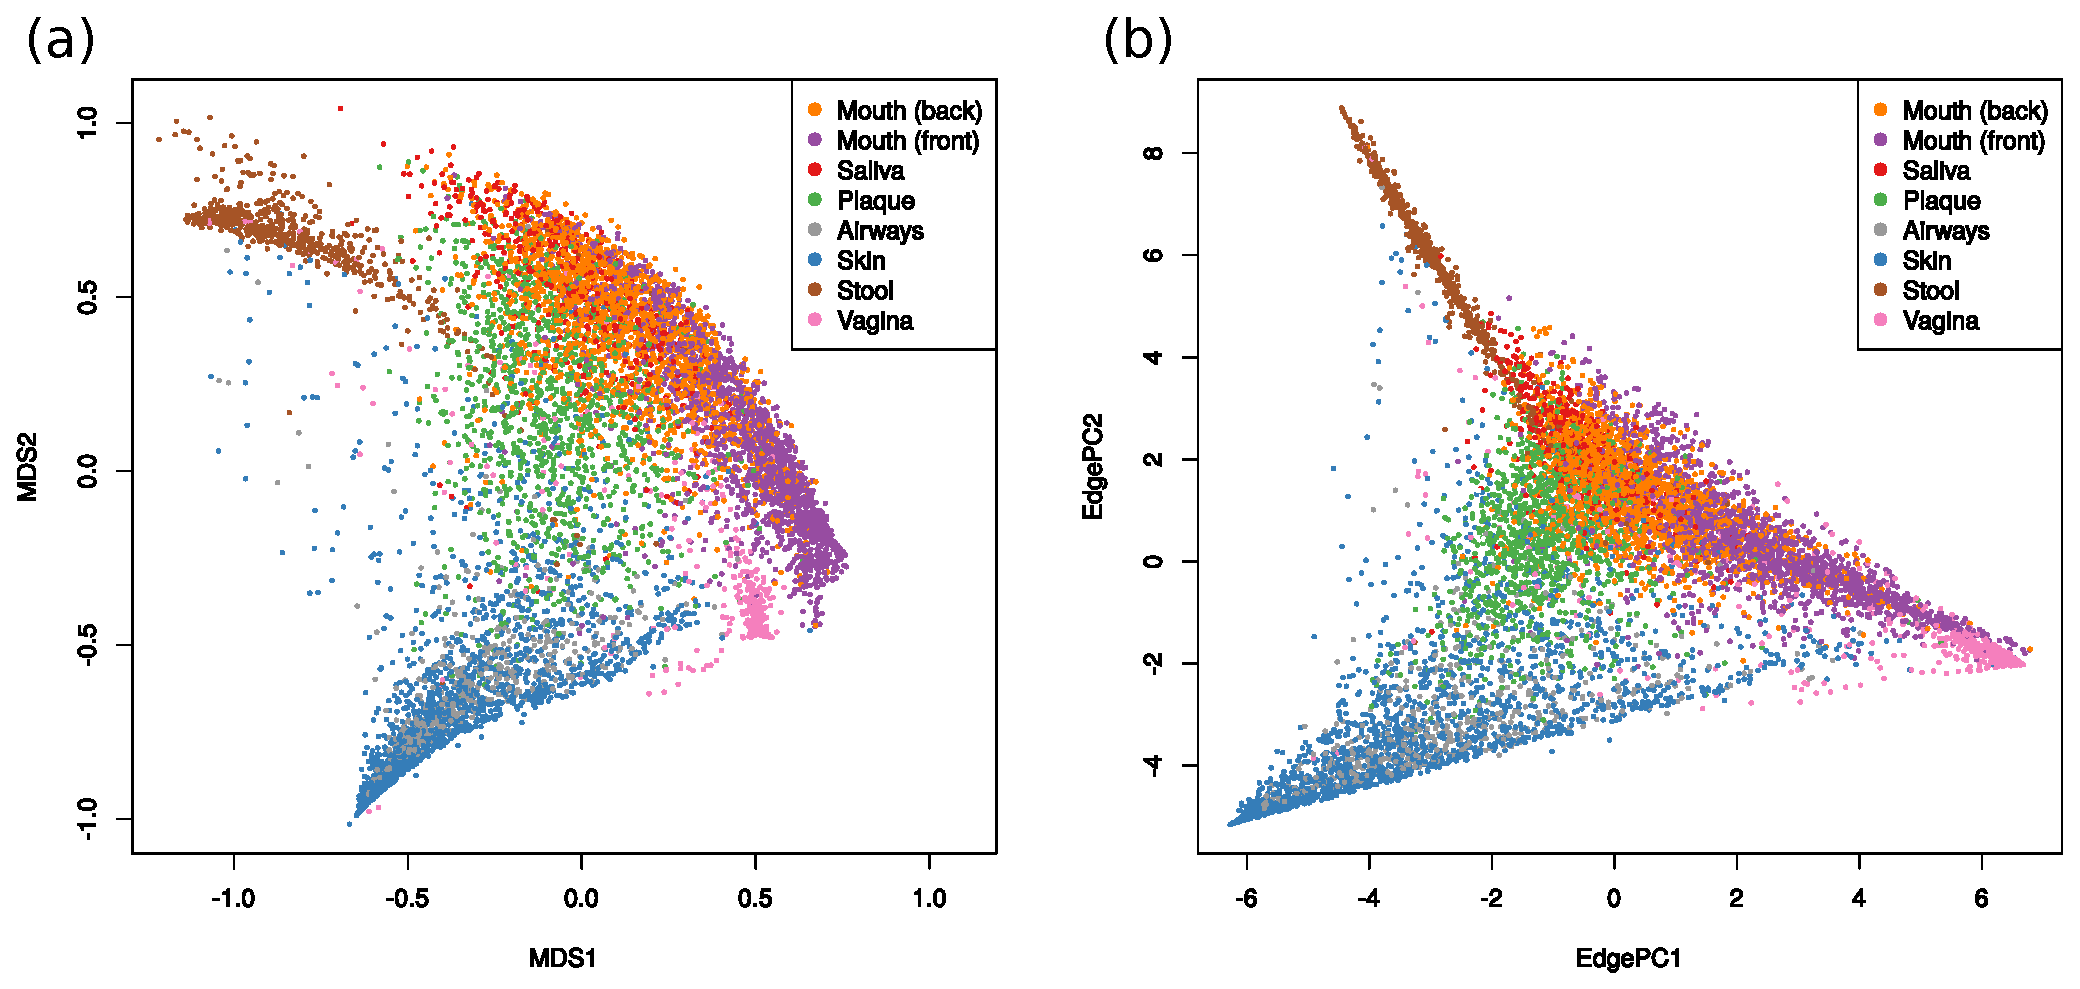
\includegraphics[width=\linewidth]{art/mds_epca.pdf}
    \begin{subfigure}{0pt}
        \phantomcaption
        \label{fig:hmp_mds_epca:sub:mds}
    \end{subfigure}
    \begin{subfigure}{0pt}
        \phantomcaption
        \label{fig:hmp_mds_epca:sub:edge_pca}
    \end{subfigure}
    \caption[Assessment of a \acs{PhAT} for large dataset analyses]{
        \textbf{Assessment of a \acs{PhAT} for large dataset analyses.}
        Here, we test the unconstrained \taxonname{Bacteria} tree generated by our \ac{PhAT} method
        for placing and analyzing a large sequence dataset.
        For this, we use the Human Microbiome Project (HMP) \citep{Huttenhower2012,Methe2012} data,
        and selected \num{9192} samples from different body sites with a total of 117 million sequences.
        For details on the processing, see \secref{ch:EmpiricalDatasets}.
        We categorized the 19 original body site labels into 8 regions, in order to make the plot more readable.
        See \tabref{tab:hmp_data_overview} for the mapping between the original labels and the ones used here.
        The sequences were placed on the tree, and subsequently analyzed with two different methods.
        Both subfigures show that the tree, despite only representing higher taxonomic levels,
        suffices to separate different body site regions from each other.
%         Even different oral regions are mostly separated, although there seems to be quite some overlap.
        \\
        In subfigure \subref{fig:hmp_mds_epca:sub:mds}, we visualized the pairwise KR distances between all samples.
        The phylogenetic Kantorovich-Rubinstein (KR) distance \citep{Matsen2011a,Evans2012} between two samples,
        also known as the Earth Mover's distance,
        measures how much placement ``mass'' has to be moved by how much along the branches of the tree
        in order to transform one sample into the other.
        It is a generalization of the UniFrac distance \citep{Lozupone2005,Lozupone2007a}.
        The high-dimensional pairwise KR distance matrix was then embedded into the plot by performing \acf{MDS}.
        \ac{MDS} \citep{Mardia1978,Krzanowski1994,Everitt2010} is a dimensionality reduction technique that
        finds an embedding of a distance matrix into lower dimensions (in this case, \num{2} dimensions)
        preserving higher dimensional distances as well as possible.
        \\
        In subfigure \subref{fig:hmp_mds_epca:sub:edge_pca}, we also perform Edge PCA \citep{Matsen2011a}
        on the samples.
        The grouping of body sites is again clearly visible with this method.
%         See \figref{fig:bv_comparison} for a short explanation of this method.
        Similar to \figref{fig:bv_edgepca:sub:edgepca_orig}, the plot forms a triangle of samples,
        roughly separated by body site regions.
    }
    \label{fig:hmp_mds_epca}
\end{figure}

% ======================================================================================================================
%     Taxonomic Assignment and Profiling
% ======================================================================================================================

\subsection{Taxonomic Assignment and Profiling}
\label{ch:AutomaticTrees:sec:Evaluation:sub:TaxonomicAssignmentProfiling}

Here, we assess how \acp{PhAT} perform when used for obtaining a taxonomic profile of a set of samples in conjunction with placement.
We emphasize though that taxonomic assignment and profiling are neither the focus of \acp{PhAT},
nor the intended standard applications of phylogenetic placement.
To perform the evaluation,
we used the \taxonname{mouse gut} data set of the 2nd \toolname{CAMI} Challenge \citep{Sczyrba2017,Bremges2018},
and phylogenetically placed the reads of the  16S locus (\num{\approx 0.08}\% of the total data)
on our constrained and unconstrained \taxonname{Bacteria} trees.
We then used this placement data to taxonomically assign the reads
based on the underlying \toolname{Silva} taxonomy of the trees,
in analogy to the method used by \toolname{Sativa} \citep{Kozlov2016}.
Unfortunately, the \toolname{CAMI} Challenge uses the \toolname{NCBI} taxonomy for the respective evaluation.
We thus had to compute a mapping between the two taxonomies, which introduces some incongruities \citep{Balvociute2017}.
The resulting per-read assignment was then used to generate a taxonomic profile of the data.

Despite only using a small fraction of the reads and despite having to use incongruent taxonomies,
our PhAT-based taxonomic profiling is in the mid-range of the tools evaluated by \toolname{CAMI}.
Therefore, our method yields reasonable accuracy for taxonomic assignment and profiling.
Note that the resolution of the assignment is limited by the taxonomy used when running the \ac{PhAT} method,
that is, we could not assign reads at \taxonname{Species} level.

% Details of the process and its results are provided in \secref{ch:AutomaticTrees:sec:Evaluation:sub:TaxonomicAssignmentProfilingDetails};

\figref{fig:cami_performance}, \figref{fig:cami_alpha_diversity}, and \tabref{tab:cami_rankings} show the most important evaluation results.

\figref{fig:cami_performance_relative} and \figref{fig:cami_performance_absolute}

details from the supplement:

Taxonomic profiling is one potential application of phylogenetic placement.
Thus, we also tested how well our \acp{PhAT} are suited for this purpose.
% To this end, we conducted CAMI Challenge \citep{Sczyrba2017}
The CAMI Challenge \citep{Sczyrba2017} is a community-driven effort to assess taxonomic profiling methods
using a common set of benchmark data sets.
To assess the feasibility of using trees generated with \ac{PhAT} to perform taxonomic profiling of microbiome data,
we utilized the \taxonname{mouse gut} data set of the 2nd CAMI Challenge \citep{Bremges2018}.
For this data set, we performed read preprocessing, phylogenetic placement
against our constrained and unconstrained \taxonname{Bacterial} trees,
and subsequent taxonomic assignment.

More specifically, we used the unpaired HiSeq reads of the mouse gut data set from CAMI,
which comprises \num{64} samples of simulated reads.
The preprocessing involved read de-interleaving following \cite{DeinterleaveFastq},
paired-end read merging using \toolname{PEAR} \citep{Zhang2014},
as well as quality filtering and conversion to \texttt{fasta} using \toolname{VSEARCH2} \citep{Rognes2016}.
This yielded a total of \num{800 341 409} reads.
As our trees are based on small ribosomal subunit sequences,
we also performed read filtering to obtain reads from the 16S rDNA locus.
This filtering was performed using the protocol of \cite{Logares2014},
which relies on \toolname{HMMER} \citep{Eddy1998,Eddy2009}, and respective profiles for the 16S rDNA locus.
We performed a global identity based de-replication step on the resulting reads that yielded \num{616 405} query sequences.
We aligned these query sequences to our \taxonname{Bacteria} reference alignment
using \toolname{PaPaRa~2.0} \citep{Berger2011a,Berger2012}.
We then performed phylogenetic placement of the aligned query sequences onto the unconstrained and constrained reference trees,
respectively, using \toolname{EPA-ng} \citep{Barbera2018}.
We performed de-de-replication to obtain per-sample data again, %on the \texttt{jplace} file,
resulting in \num{64} \texttt{jplace} files (one per original sample) with placements of the 16S rDNA sequences,
for each of the two trees.

Finally, we performed taxonomic assignment and taxonomic profiling of the per-sample results
using the \texttt{assign} command implemented in \toolname{gappa},
which works analogously to the method used in \toolname{Sativa} \citep{Kozlov2016}.
Its basic steps are described in \secref{ch:PipelineImplementation}.
The CAMI challenge requires taxonomic assignments
that conform with the \toolname{NCBI} taxonomy \citep{Sayers2009,Benson2009}.
As our reference tree is however based on the \toolname{Silva} taxonomy \citep{Yilmaz2014},
we developed a dedicated mapping procedure to, in a best effort approach,
map our results to \toolname{NCBI} taxonomic names and IDs.
The mapping is based on the \textit{loose mapping} procedure by \cite{Balvociute2017}.
More specifically, we try to map taxonomic paths to their name, rank, and ID in the \toolname{NCBI} taxonomy,
if we find a name-based match between the two.
When this fails, the phylogenetic placement mass assigned to a taxonomic path by our approach
is instead added to the last successful mapping further up in the taxonomic hierarchy.
By initiating this procedure for each taxonomic path from its root downwards,
we ensure that all placement masses are taken into account.

This mapping is a major disadvantage of our approach when using a \toolname{Silva}-based reference,
as the \toolname{Silva} and \toolname{NCBI} taxonomies are far from being congruent \citep{Balvociute2017}.
Also note that our reference is limited to 16S rDNA locus. This substantially reduces the volume of data we can evaluate.
In this particular test, only \num{\approx 0.08}\% of the total data was identified as belonging to 16S.
This means that our taxonomic profiling only uses a small fraction of the available data.
% that is, for estimating relative fractions of the taxa present in the data.

Finally, we used the CAMI evaluation tool for taxonomic profilers, OPAL \citep{Sczyrba2017},
to compare our approach to competing software and the ``gold standard'' result for the data set.
Despite the aforementioned caveats of taxonomic profiling using phylogenetic placements in the CAMI setting,
we find that the performance of our approach is ``middle of the field''.
Note that this is a comparison to tools that are dedicated to taxonomic profiling,
which also typically can assign more of the available reads.

We show the most important OPAL results in \figref{fig:cami_performance}, \figref{fig:cami_alpha_diversity},
as well as in \tabref{tab:cami_rankings}.
Furthermore, the full OPAL output can be accessed at \url{http://github.com/lczech/placement-methods-paper}.



\afterpage{
\begin{landscape}
\begin{table}[htb]
\caption[CAMI: Scores and Ranks]{
\textbf{CAMI: Scores and Ranks.}
The table shows the scores and ranks of different tools evaluated with data from, and following the protocol of,
the 2nd CAMI challenge \citep{Sczyrba2017,Bremges2018}.
Here, we compare the taxonomic assignment and profiling conducted with our \texttt{assign} command
to the tools that took part in the 2nd CAMI challenge.
For this, we used the unconstrained and constrained \taxonname{Bacterial} tree,
which are abbreviated in the table as ``PhAT (U)'' and ``PhAT (C)'', respectively.
See \secref{ch:AutomaticTrees:sec:Evaluation:sub:TaxonomicAssignmentProfiling} for details.
\\
Four metrics are used in CAMI for evaluating tools:
Recall (completeness), precision (purity), L1 norm error (abbreviated here as L1 NE),
and Weighted Unifrac Error (abbreviated here as WUE).
For each metric, the comparative scores of the tools are shown, as well as their rankings, relative to each other.
Also, the total sum of scores and the total rank are shown, which add up the values of the four metrics.
The procedure of the scoring and ranking is explained in detail in the Online Supplement of \cite{Sczyrba2017}.
\\
Despite the caveats and limitations that are explained in \secref{ch:AutomaticTrees:sec:Evaluation:sub:TaxonomicAssignmentProfiling},
using our \acp{PhAT} trees to obtain a taxonomic profile yields rankings in the middle of the field for all metrics.
}
\label{tab:cami_rankings}
{
    \begin{center}
    \begin{tabular}{lrrrrrrrrrr}
        \toprule
                       & \multicolumn{2}{c}{Total} & \multicolumn{2}{c}{Recall} & \multicolumn{2}{c}{Precision} & \multicolumn{2}{c}{L1 NE} & \multicolumn{2}{c}{WUE} \\
        Tool           & Sum & Rank & Score & Rank & Score & Rank & Score & Rank & Score & Rank \\
        \midrule
        Metaphlan           &   1814    &   1   &   958     &   3   &  75       &   1   &  731      &   2   & 50    &   1   \\
        MetaPhyler          &   2995    &   2   &   314     &   1   &  2119     &   7   &  322      &   1   & 240   &   5   \\
        CommonKmers         &   3333    &   3   &   1448    &   6   &  409      &   2   &  1318     &   7   & 158   &   3   \\
        mOTU                &   3751    &   4   &   1703    &   8   &  488      &   3   &  1260     &   5   & 300   &   6   \\
        \textbf{PhAT (C)}   &   3784    &   5   &   1202    &   4   &  1116     &   4   &  1280     &   6   & 186   &   4   \\
        \textbf{PhAT (U)}   &   3933    &   6   &   1436    &   5   &  1153     &   5   &  1208     &   4   & 136   &   2   \\
        TIPP                &   4263    &   7   &   892     &   2   &  2126     &   8   &  930      &   3   & 315   &   7   \\
        FOCUS               &   6153    &   8   &   2079    &   9   &  1636     &   6   &  2018     &   8   & 420   &   8   \\
        Quikr               &   6838    &   9   &   1488    &   7   &  2398     &   9   &  2453     &   9   & 499   &   9   \\
        \bottomrule
    \end{tabular}
    \end{center}
}
\end{table}
\end{landscape}
} %afterpage

% \begin{table}[htb]
% \caption{
% \textbf{CAMI Rankings.}
% The table shows the rankings of different tools evaluated with CAMI...
% }
% \label{tab:cami_rankings}
% {
%     \begin{center}
%     \begin{tabular}{lrlrlrlrlr}
%         \toprule
%         Sum of Scores & & Completeness (recall) & & Purity (precision) & & L1 Norm Error & & Weighted Unifrac Error \\
%         \midrule
%         Metaphlan   & 1605 & MetaPhyler  & 236  & Metaphlan     & 75   & MetaPhyler     & Metaphlan     & 37  \\
%         MetaPhyler  & 2561 & TIPP        & 788  & CommonKmers   & 406  & Metaphlan      & \PhAT         & 127 \\
%         CommonKmers & 2952 & Metaphlan   & 868  & mOTU          & 487  & TIPP           & CommonKmers   & 130 \\
%         \PhAT       & 3311 & \PhAT       & 1145 & \PhAT         & 970  & \PhAT          & MetaPhyler    & 195 \\
%         mOTU        & 3321 & CommonKmers & 1265 & FOCUS         & 1338 & mOTU           & mOTU          & 244 \\
%         TIPP        & 3667 & Quikr       & 1290 & MetaPhyler    & 1800 & CommonKmers    & TIPP          & 261 \\
%         FOCUS       & 5310 & mOTU        & 1501 & TIPP          & 1806 & FOCUS          & FOCUS         & 363 \\
%         Quikr       & 5945 & FOCUS       & 1840 & Quikr         & 2078 & Quikr          & Quikr         & 435 \\
%         \bottomrule
%     \end{tabular}
%     \end{center}
% }
% \end{table}

% Landscape table
% https://tex.stackexchange.com/a/19021
% \afterpage{%
% \clearpage% Flush earlier floats (otherwise order might not be correct)
% %     \thispagestyle{empty}% empty page style (?)
% \begin{landscape}% Landscape page
%     \centering % Center table
%     \begin{table}[htb]
%     \caption{
%     \textbf{CAMI Rankings.}
%     The table shows the rankings of different tools evaluated with CAMI...
%     }
%     \label{tab:cami_rankings}
%     {
%         \begin{center}
%         \begin{tabular}{lrlrlrlrlr}
%             \toprule
%             Sum of Scores & & Completeness (recall) & & Purity (precision) & & L1 Norm Error & & Weighted Unifrac Error \\
%             \midrule
%             Metaphlan      & 1605 & MetaPhyler     & 236  & Metaphlan        & 75   & MetaPhyler        & 303  & Metaphlan        & 37  \\
%             MetaPhyler     & 2561 & TIPP           & 788  & CommonKmers      & 406  & Metaphlan         & 625  & \textbf{\PhAT}   & 127 \\
%             CommonKmers    & 2952 & Metaphlan      & 868  & mOTU             & 487  & TIPP              & 812  & CommonKmers      & 130 \\
%             \textbf{\PhAT} & 3311 & \textbf{\PhAT} & 1145 & \textbf{\PhAT}   & 970  & \textbf{\PhAT}    & 1069 & MetaPhyler       & 195 \\
%             mOTU           & 3321 & CommonKmers    & 1265 & FOCUS            & 1338 & mOTU              & 1089 & mOTU             & 244 \\
%             TIPP           & 3667 & Quikr          & 1290 & MetaPhyler       & 1800 & CommonKmers       & 1151 & TIPP             & 261 \\
%             FOCUS          & 5310 & mOTU           & 1501 & TIPP             & 1806 & FOCUS             & 1769 & FOCUS            & 363 \\
%             Quikr          & 5945 & FOCUS          & 1840 & Quikr            & 2078 & Quikr             & 2142 & Quikr            & 435 \\
%             \bottomrule
%         \end{tabular}
%         \end{center}
%     }
%     \end{table}
% \end{landscape}
% \clearpage% Flush page
% }

% -----------------------------------------
%     CAMI Performance
% -----------------------------------------

\begin{figure}[hpbt]
    \centering
    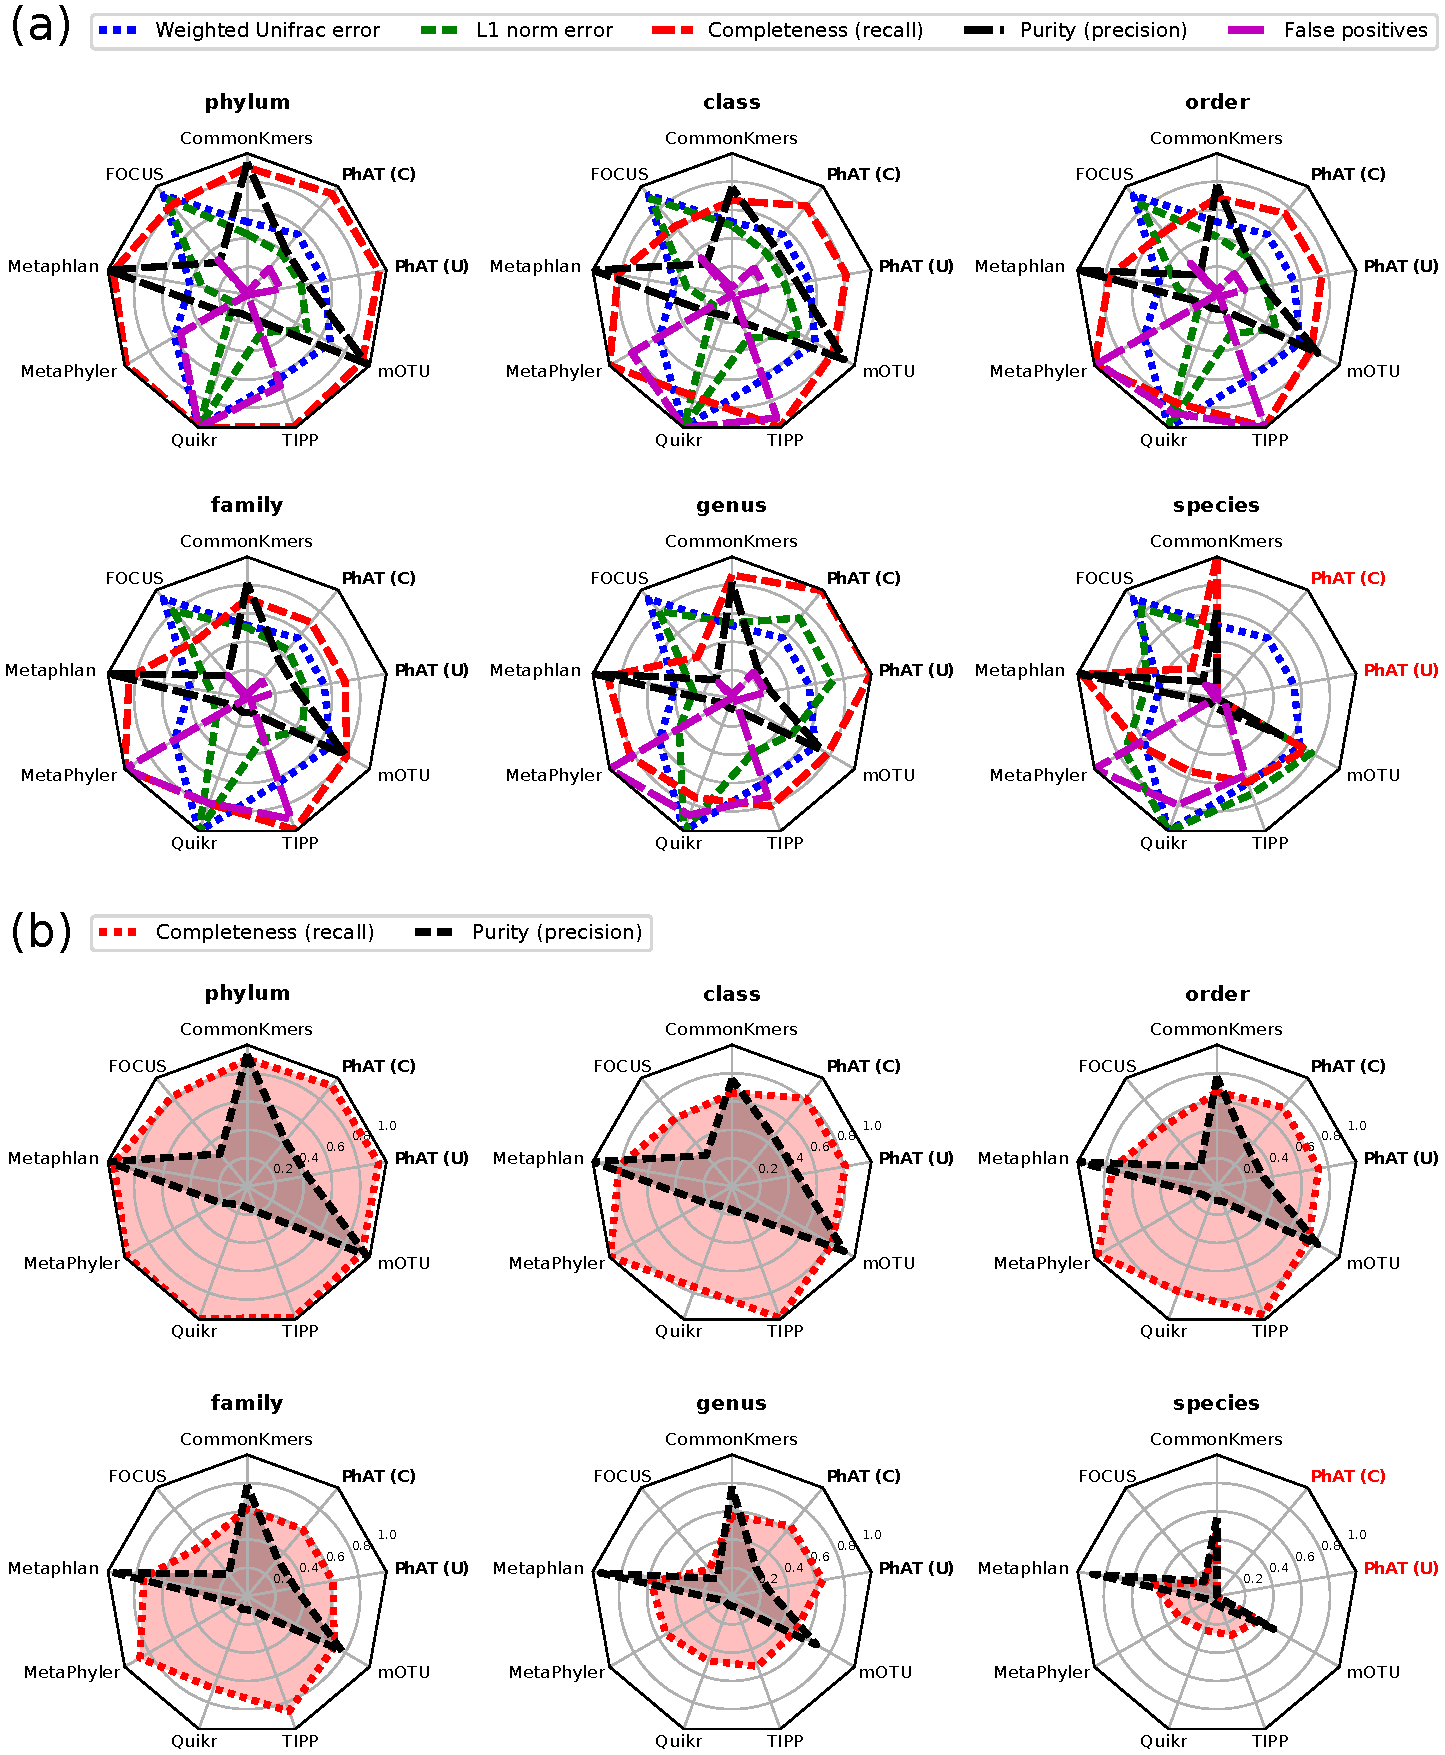
\includegraphics[width=0.94\linewidth]{art/cami_performance.pdf}
    \begin{subfigure}{0pt}
        \phantomcaption
        \label{fig:cami_performance:sub:relative}
    \end{subfigure}
    \begin{subfigure}{0pt}
        \phantomcaption
        \label{fig:cami_performance:sub:absolute}
    \end{subfigure}
    \caption[CAMI: Profiling Results]{
        \textbf{CAMI: Profiling Results.}
        The figure shows the profiling results of different tools evaluated with data from, and following the protocol of,
        the 2nd CAMI challenge \citep{Sczyrba2017,Bremges2018}.
        Here, we compare the taxonomic assignment and profiling conducted with our \texttt{assign} command
        to the tools that took part in the 2nd CAMI challenge.
        For this, we used the unconstrained and constrained \taxonname{Bacterial} tree,
        which are abbreviated here as ``PhAT (U)'' and ``PhAT (C)'', respectively.
        See \secref{ch:AutomaticTrees:sec:Evaluation:sub:TaxonomicAssignmentProfiling} for details on our evaluation,
        and see \cite{Sczyrba2017} for details on CAMI and their metrics.
        \\
%         Subfigure \subref{fig:cami_performance:sub:relative} shows the relative performance of the tools
%         for different taxonomic ranks by displaying the error metrics used by CAMI:
%         Weighted Unifrac error, L1 norm error, recall (completeness), precision (purity) and false positives.
%         The error metrics were divided by their respective maximal value to allow viewing them on the same scale
%         and to allow relative performance comparisons.
%         \\
%         Subfigure \subref{fig:cami_performance:sub:absolute} shows the absolute recall (completeness) and precision (purity)
%         for each tool across the taxonomic ranks.
%         \\
        In both subfigures, the red text for our PhAT evaluations indicates
        that no predictions at the corresponding taxonomic rank were returned.
        This is because our \toolname{Silva}-based tree does not have \taxonname{species} resolution
        and does hence not allow for taxonomic profiling at this level.
    }
    \label{fig:cami_performance}
\end{figure}

% -----------------------------------------
%     CAMI Relative Performance
% -----------------------------------------

\begin{figure}[hpbt]
    \centering
    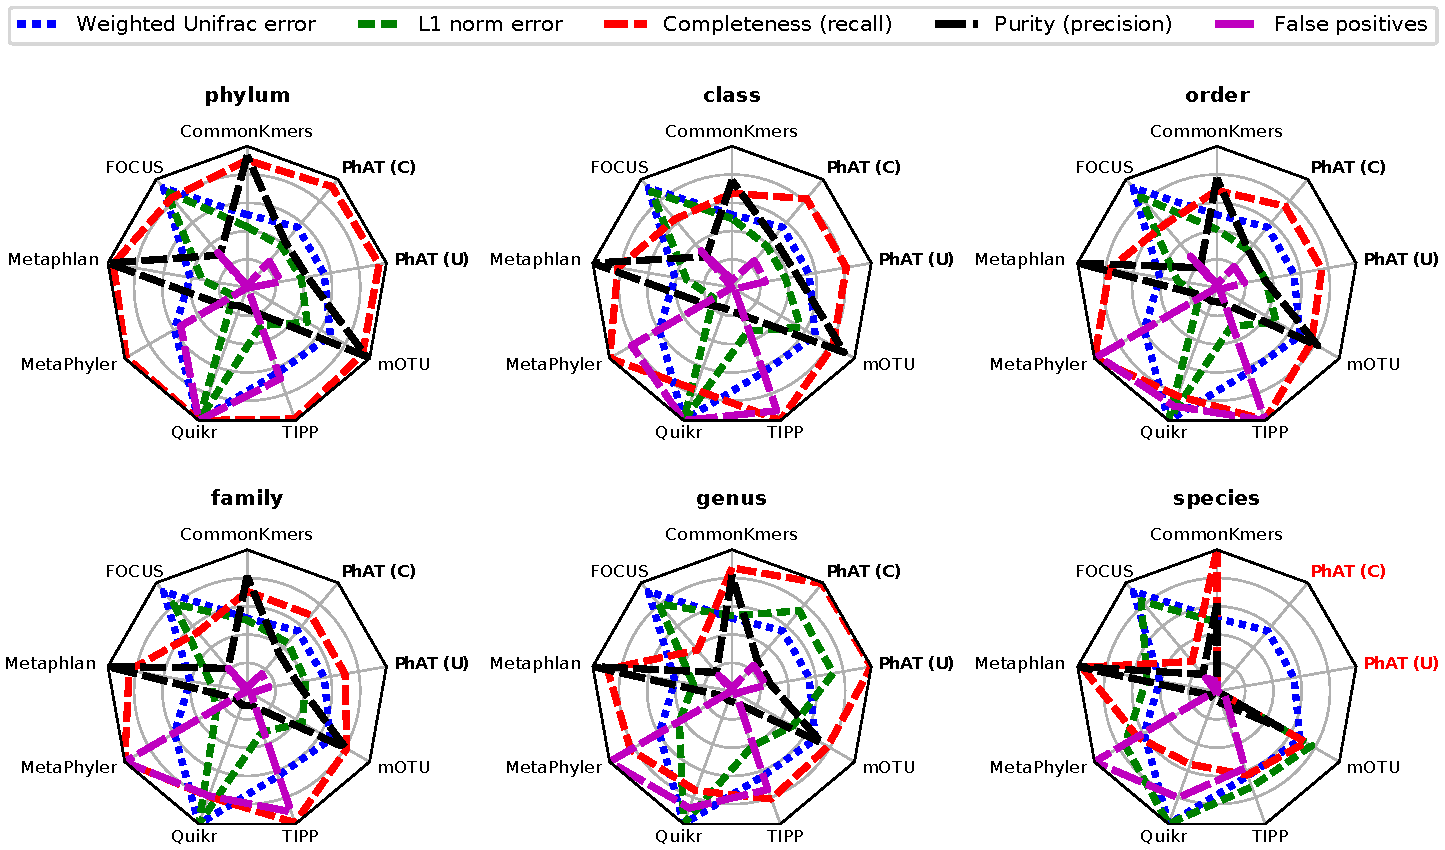
\includegraphics[width=\linewidth]{cami_performance_relative.pdf}
    \vspace{1em}
    \caption[CAMI: Relative Performance]{
        \textbf{CAMI: Relative Performance.}
        The Figure shows the relative performance of the tools
        for different taxonomic ranks by displaying the error metrics used by CAMI:
        Weighted Unifrac error, L1 norm error, recall (completeness), precision (purity) and false positives.
        The error metrics were divided by their respective maximal value to allow viewing them on the same scale
        and to allow relative performance comparisons.
    }
    \label{fig:cami_performance_relative}
\end{figure}

% -----------------------------------------
%     CAMI Absolute Performance
% -----------------------------------------

\begin{figure}[hpbt]
    \centering
    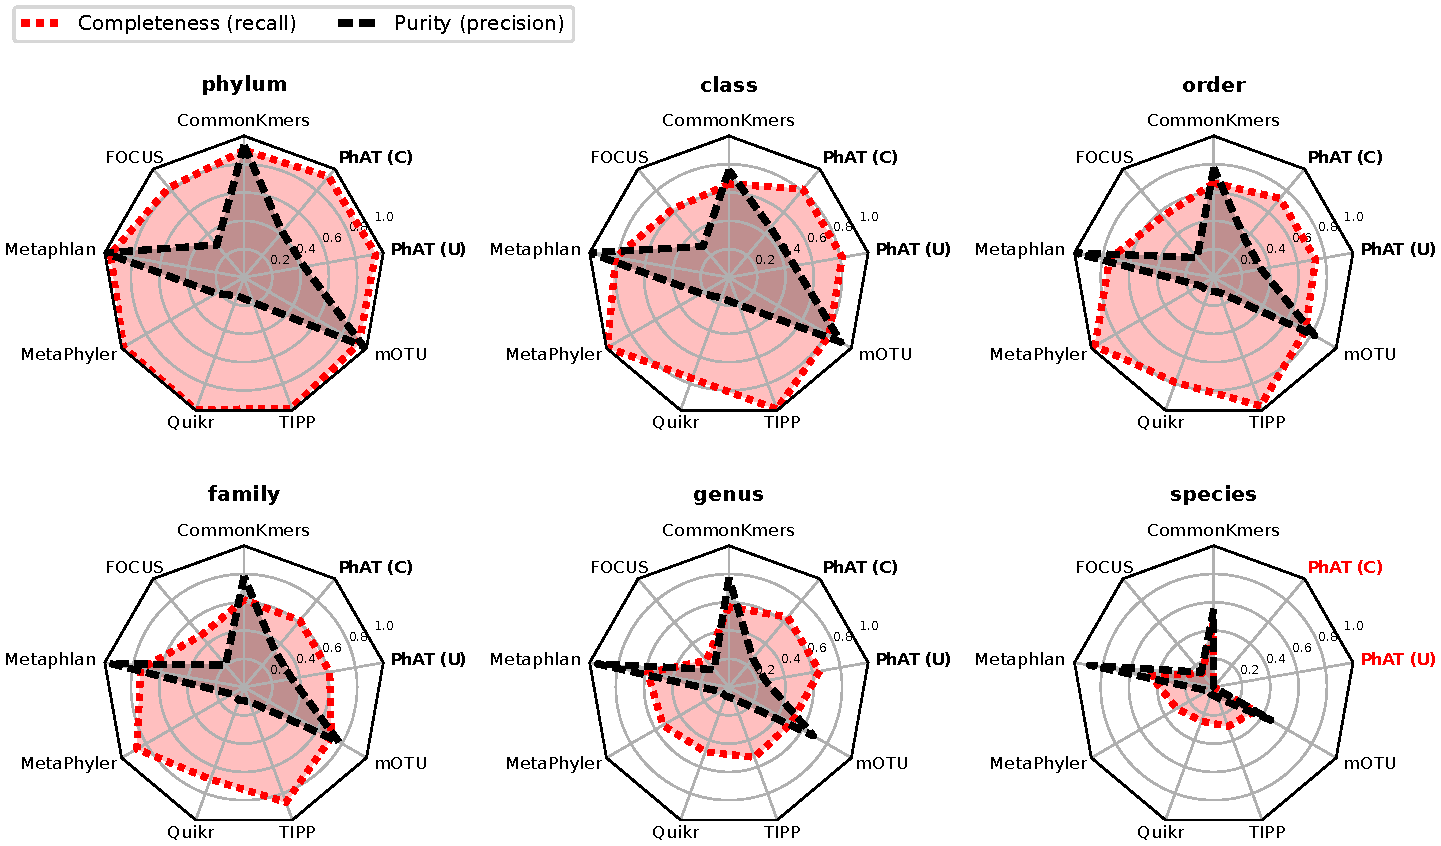
\includegraphics[width=\linewidth]{cami_performance_absolute.pdf}
    \vspace{1em}
    \caption[CAMI: Absolute Performance]{
        \textbf{CAMI: Absolute Performance.}
        The Figure shows the absolute recall (completeness) and precision (purity)
        for each tool across the taxonomic ranks.
    }
    \label{fig:cami_performance_absolute}
\end{figure}

% -----------------------------------------
%     CAMI Alpha Diversity
% -----------------------------------------

\begin{figure}[hpbt]
    \centering
    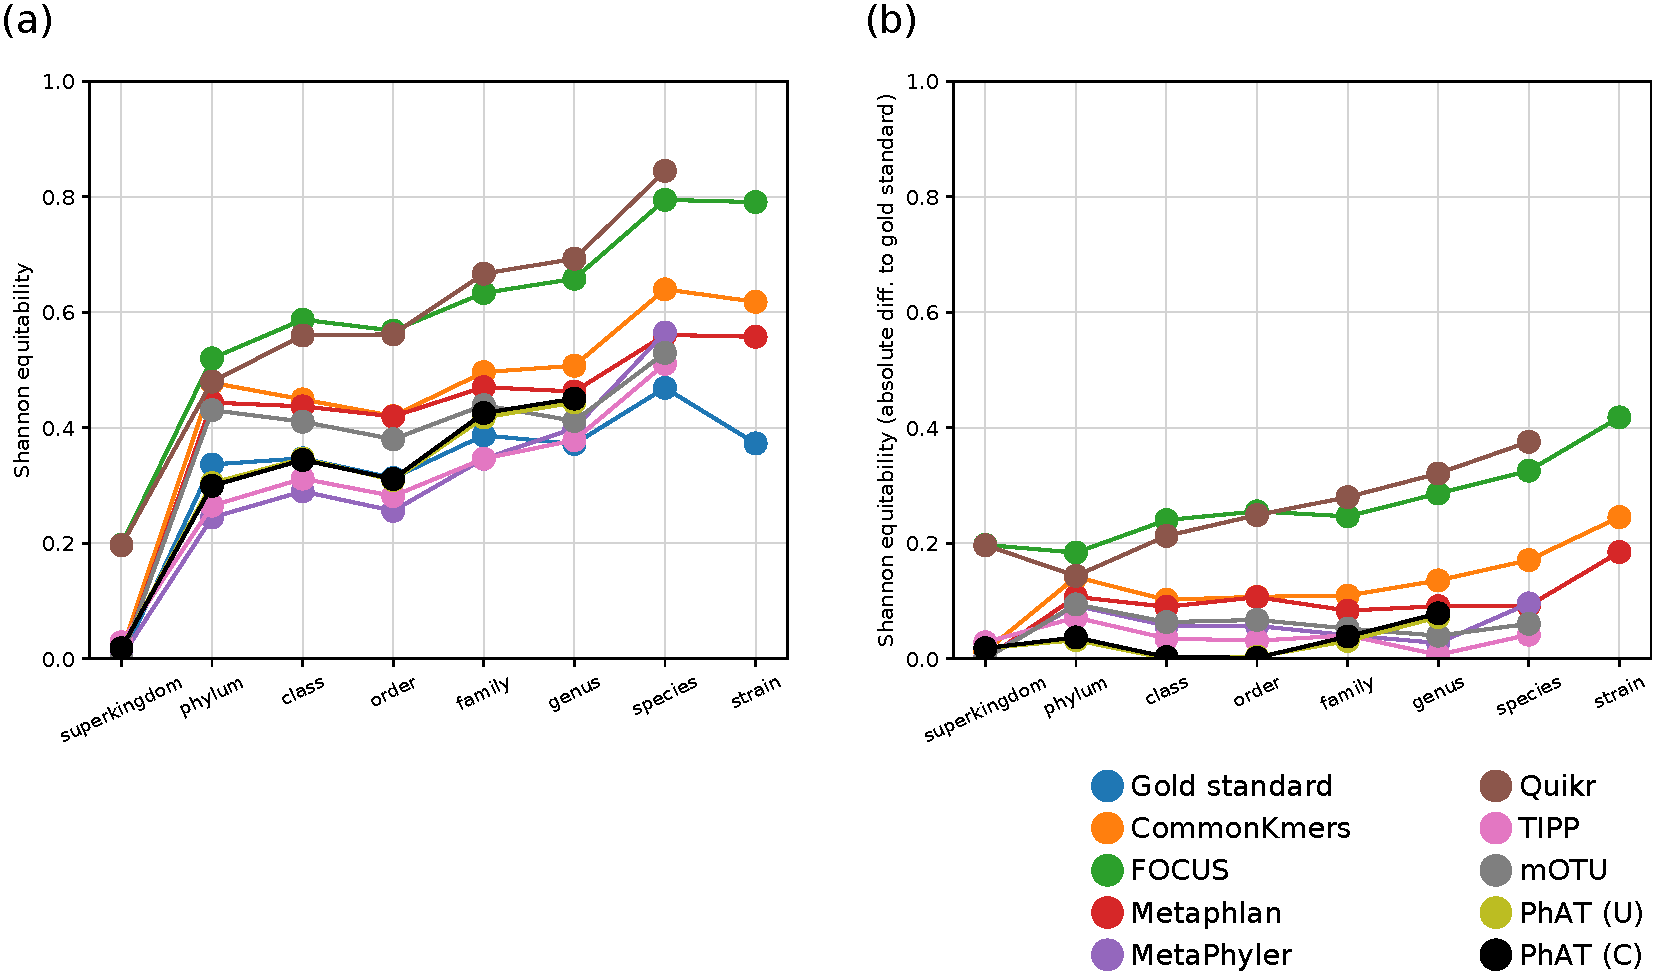
\includegraphics[width=\linewidth]{cami_alpha_diversity.pdf}
    \begin{subfigure}{0pt}
        \phantomcaption
        \label{fig:cami_alpha_diversity:sub:total}
    \end{subfigure}
    \begin{subfigure}{0pt}
        \phantomcaption
        \label{fig:cami_alpha_diversity:sub:difference}
    \end{subfigure}
    \caption[CAMI: Alpha Diversity]{
        \textbf{CAMI: Alpha Diversity.}
        The figure shows the alpha diversity as estimated by different tools evaluated
        with data from, and following the protocol of, the 2nd CAMI challenge \citep{Sczyrba2017,Bremges2018}.
        Here, we compare the taxonomic assignment and profiling conducted with our \texttt{assign} command
        to the tools that took part in the 2nd CAMI challenge.
        For this, we used the unconstrained and constrained \taxonname{Bacterial} tree,
        which are abbreviated here as ``PhAT (U)'' and ``PhAT (C)'', respectively.
%         See Supplementary Section~\ref{sec:TaxonomicAssignment} for details.
%         \\
        \todo{add some more text here}
    }
    \label{fig:cami_alpha_diversity}
\end{figure}

% ======================================================================================================================
%     Multilevel Placement
% ======================================================================================================================

\subsection{Subclades and Multilevel Placement}
\label{ch:AutomaticTrees:sec:Evaluation:sub:MultilevelPlacement}

We selected five bacterial clades to evaluate \ac{PhAT} accuracy on smaller clades,
as well as to assess some properties of the Multilevel Placement approach.
The same clades were already scrutinized in \toolname{Sativa} \citep{Kozlov2016}.
\figref{fig:clades} shows the \taxonname{Bacteria} tree with the five test clades highlighted.

% \section{Evaluation of Multilevel Placement}
% \label{sec:EvaluationMultilevelPlacement}

\begin{figure}[hpbt]
    \centering
    \includegraphics[width=\linewidth]{art/clades.pdf}
    \vspace*{0.5em}
    \caption[Unconstrained \taxonname{Bacteria} tree with five bacterial sub-clades]{
        \textbf{Unconstrained \taxonname{Bacteria} tree with five bacterial sub-clades.}
        This tree is the result of our \ac{PhAT} method
        applied to the \taxonname{Bacteria} sequences in \toolname{Silva}.
        The tree contains a total of 1914 taxa.
        Colorized are the five \taxonname{Phylum} level sub-clades that we used for testing multilevel placement:
        \taxonname{Proteobacteria} (505 taxa), \taxonname{Bacteroidetes} (362 taxa), \taxonname{Firmicutes} (360 taxa),
        \taxonname{Cyanobacteria} (39 taxa) and \taxonname{Actinobacteria} (53 taxa).
        The incongruence between taxonomy and phylogeny is visible here as non-monophyletic colored branches.
        We thus here define a clade to consist of all branches
        that are part of a monophyletic split of the tree with respect to the taxa in the clade.
        In other words, all branches on one side of a split are considered to belong to a clade,
        if that side of the split only contains taxa from that clade.
        These branches then receive the same color here.
        Then, for multilevel placement, a sequence is considered to be part of a clade
        if its most probable placement falls into that clade.
        For example, a sequence that is placed onto one of the orange branches on this tree
        is subsequently placed in the \taxonname{Cyanobacteria} tree for the second level placement.
        Each of the five sub-clades is represented by multiple branches here,
        which we call the ``overlap'' with the \taxonname{Bacteria} tree.
    }
    \label{fig:clades}
\end{figure}

\todo{add a table to the supplement that lists which of our five test clades contains how many seqs in the backbone
and how many in the second level alignments.}
\todo{list how many taxa the general tree has for each clade, and how big each clade tree is -- that is, list the number of overlapping taxa.}
\todo{table of tree sizes? see supp fig}

\paragraph{Subclade Accuracy}
\label{ch:AutomaticTrees:sec:Evaluation:sub:MultilevelPlacement:par:SubcladeAccuracy}

First, using the sequences and taxonomies of these five clades, we built unconstrained and constrained \acp{PhAT}.
We then conducted the same accuracy analysis as explained before on these ten trees.
That is, we placed the \toolname{Silva} sequences of the five clades onto their respective \ac{PhAT}
and evaluated distances to expected branches.
Thereby, we evaluated the accuracy of these \acp{PhAT} when used as second level \aclp{CT}.
The results are shown in \figref{fig:multilevel}.
The placement accuracy is slightly worse for the clade trees than for the eight comprehensive \acp{PhAT} evaluated before.
This is again likely due to 16S SSU sequences being unable to properly resolve lower taxonomic levels \citep{Janda2007}.

\begin{figure}[hpbt]
    \centering
    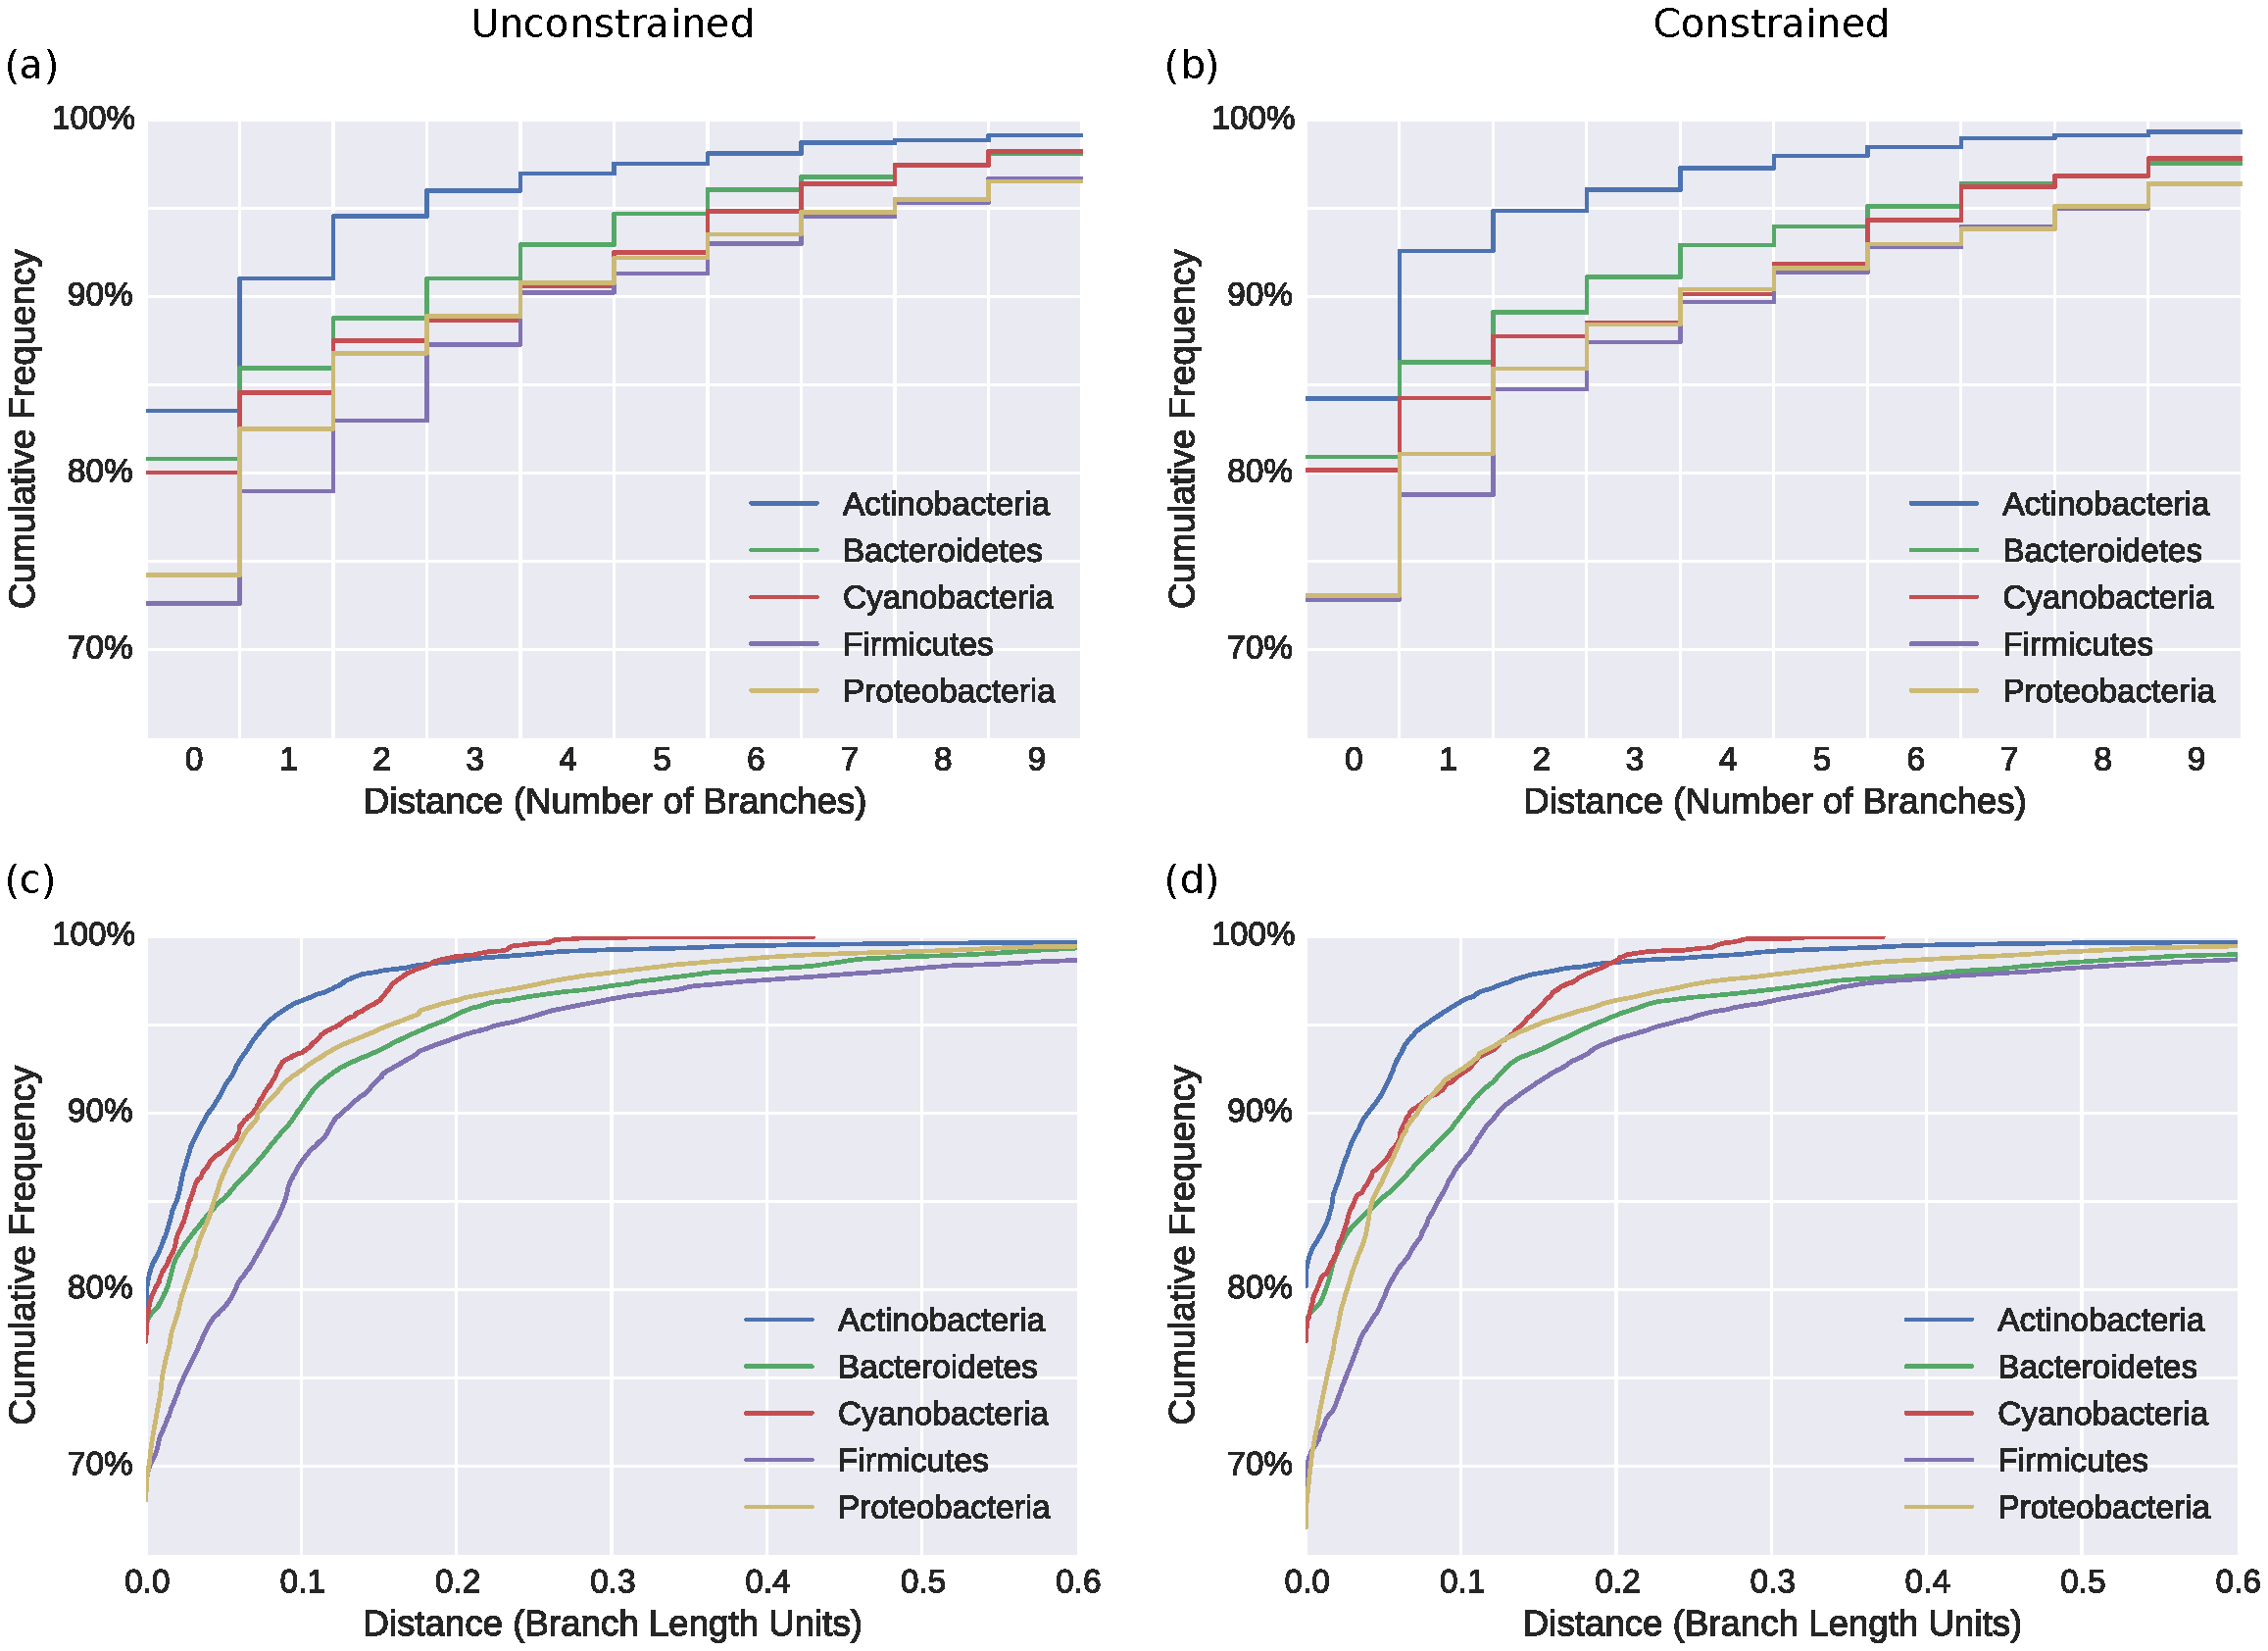
\includegraphics[width=\linewidth]{art/multilevel.pdf}
    \begin{subfigure}{0pt}
        \phantomcaption
        \label{fig:multilevel:sub:edge_unconstr}
    \end{subfigure}
    \begin{subfigure}{0pt}
        \phantomcaption
        \label{fig:multilevel:sub:edge_constr}
    \end{subfigure}
    \begin{subfigure}{0pt}
        \phantomcaption
        \label{fig:multilevel:sub:branch_unconstr}
    \end{subfigure}
    \begin{subfigure}{0pt}
        \phantomcaption
        \label{fig:multilevel:sub:branch_constr}
    \end{subfigure}
    \caption[Accuracy of the \acsp{PhAT} of five bacterial sub-clades]{
        \textbf{Accuracy of the \acsp{PhAT} of five bacterial sub-clades.}
        We used five sub-clades of the \taxonname{Bacteria} in \toolname{Silva},
        which were already scrutinized in \citep{Kozlov2016},
        to test how our \ac{PhAT} method works for less diverse sets of sequences.
        These five clades are also highlighted in \figref{fig:clades};
        see there for a description of the clades.
        The evaluation was conducted as explained in the text;
        \todo{and follows the accuracy measurement as explained in sec and fig...}
        in short, we placed the \toolname{Silva} sequences of the clades on their respective tree,
        and measured how far each of them is away from the branch of the consensus sequence it is represented by.
%         The figure follows \figref{fig:constraints_backbone} in layout.
    }
    \label{fig:multilevel}
\end{figure}

% from top eval in /home/lucas/Projects/bacardi/02\_multilevel/05\_accuracy\_viz
% Actinobacteria  Correct pqueries 0: 41590 / 50700 = 0.820316
% Cyanobacteria   Correct pqueries 0: 8901 / 11180 = 0.796154
% Proteobacteria  Correct pqueries 0: 138944 / 195517 = 0.710649
% Firmicutes      Correct pqueries 0: 98417 / 138460 = 0.710797
% Bacteroidetes   Correct pqueries 0: 38924 / 49144 = 0.79204
% total                               326776      445001      0.7343264397

% for mean genera listing, see  02_multilevel/06_mean_genera

% Subtree Phyla
% ==========================
%
% Cyanobacteria
% 94 taxa
% 11,379 sequences
%
% Proteobacteria
% 1,569 taxa
% 200,083 sequences
%
% Firmicutes
% 652 taxa
% 138,636 sequences
%
% Bacteroidetes
% 440 taxa
% 49,214 sequences
%
% Actinobacteria
% 494 taxa
% 51,160 sequence

from the fig:

The placement accuracy on these sub-clades is slightly worse compared to the broad \taxonname{Bacteria} tree,
which can be seen by comparison to \figref{fig:constraints_backbone}.
On average, 73.4\% of the sequences were placed exactly on their expected branch,
dominated by \taxonname{Proteobacteria} and \taxonname{Firmicutes},
which combined make up 75\% of the sequences in the five clades, and have an accuracy of 71\%.
The \taxonname{Actinobacteria} have the highest accuracy,
with 82\% of their sequences placed on the expected branch.

% There are however also differences between the clades.
The two smallest clades, \taxonname{Actinobacteria} and \taxonname{Cyanobacteria},
exhibit the shortest distances in branch length units.
In fact, the longest distance of any sequence from its expected branch in the \taxonname{Cyanobacteria} clade
is around \num{0.4}, which is indicated by the end of the red line in the lower two plots.
On the other hand, the \taxonname{Firmicutes} generally have the lowest accuracy here.
In \figref{fig:clades}, which shows the unconstrained \taxonname{Bacteria} tree,
the \taxonname{Firmicutes} clade exhibits many paraphyletic branches,
which is a known issue \citep{Parks2018}.
This indicates that there is a high incongruence
between the \taxonname{Firmicutes} taxonomy and phylogeny in \toolname{Silva},
which might explain why the \taxonname{Firmicutes} score worst here.

These results are likely due to the inability of 16S SSU sequences to properly resolve lower taxonomic levels
\citep{Mignard2006,Petti2007,Janda2007}.
For example, Table 2 of \citep{Janda2007} lists \num{10} bacterial genera
that are known to be hard to identify using 16S sequences.
These genera account for \num{7.9}\% of the \num{2846} taxa
that are represented by the five bacterial trees tested here.
Furthermore, \num{95 553} of the \num{450 313} sequences that were placed on those trees (\num{21.2}\%)
belong to one of these genera.
This might explain the worse scores of these clade trees.
Lastly, the consensus sequences at the tips of the trees represent the \taxonname{Genus} level.
Thus, these have short branches, which increases the probability of misplacements.
% the Cyanobacteria (red) ends, because there are no more placements further away from their correct edges than this.
% this shows short branches etc. get avg branch lenghts of those trees!
% number of taxa, number of sequences for each tree!
%
% and to give an example of how multilevel placement works.
% we do not trust species level placement anyway. see text

---


\paragraph{First Level Accuracy}
\label{ch:AutomaticTrees:sec:Evaluation:sub:MultilevelPlacement:par:FirstLevelAccuracy}

Next, using the five clades, we evaluated the accuracy of the first placement level when conducting Multilevel Placement.
So far, our evaluation focused on the distance from a sequence placement to its expected placement branch.
For the first placement level on a \acf{BT}, it is however more important that a sequence is placed into the correct clade.
% so that it can subsequently be placed on the correct second level \acf{CT} tree.
Thus, we used the unconstrained \taxonname{Bacteria} \ac{BT} again,
and assessed how many sequences were placed in the clades shown in \figref{fig:clades}.
Of the \num{450 313} sequences in \toolname{Silva} in these clades, % that belong to one of these clades,
98.0\% were placed (most likely placement) into a branch of their corresponding clade.
Thus, for multilevel placement, they will be assigned to the correct second level \acf{CT}.
% This is expected, as these clades represent high taxonomic ranks. % everything else would mean that EPA is not doing anything reasonable at all...
More specifically, the \taxonname{Firmicutes} perform worst,
as only 94.7\% of the \taxonname{Firmicute} sequences are placed into the corresponding clade.
This can be explained by the high amount of paraphyletic branches of this clade, cf.~\figref{fig:multilevel},
which is a known issue \citep{Parks2018}. % found a fitting fresh preprint thanks to Alexey!
The sequences of the other four clades we tested achieve a clade identification accuracy exceeding 99\%.
% This shows that having a high overlap of the clades with with the \ac{BT} yields high accuracy.
% In other words, second level clade trees should be represented by multiple branches on the backbone tree.
% We already used this in \citep{Mahe2017}.

% how many sequences were placed in the expected clades?
% from /home/lucas/Projects/bacardi/11_consensus_seqs/06_subclades
% Bacteria_Actinobacteria_:   51035   /   51160   =   0.997557
% Bacteria_Firmicutes_:       131213  /   138517  =   0.94727
% Bacteria_Proteobacteria_:   199121  /   200083  =   0.995192
% Bacteria_Bacteroidetes_:    48788   /   49174   =   0.99215
% Bacteria_Cyanobacteria_:    11316   /   11379   =   0.994463
% total                      441473   /   450313  =   0.9803692099

As mentioned before, %in the method description,
a high-level taxonomic constraint can improve the accuracy of placing a sequence into the correct \ac{BT} clade.
To show this, we inferred the \taxonname{Bacteria} \ac{RT} again,
but used a \taxonname{Phylum} level constraint
% that separates the sequences of the five clades from each other and from the rest of the sequences.
that separates the five clades from each other and from the rest of the tree.
All branches within the clades were resolved using maximum likelihood.
The tree (not shown)  is similar to the tree in \figref{fig:clades}, but all five clades are now monophyletic.
Using this tree, 99.3\% of the sequences were placed into the correct clade.
Particularly the accuracy for \taxonname{Firmicutes} improved, yielding an accuracy of 99.5\%.

% 02_bact_clade_constraint/03_eval/eval.log
% Bacteria_Actinobacteria_:   50995   /   51160   =   0.996775
% Bacteria_Firmicutes_:   137839  /   138517  =   0.995105
% Bacteria_Proteobacteria_:   198320  /   200083  =   0.991189
% Bacteria_Bacteroidetes_:    48797   /   49174   =   0.992333
% Bacteria_Cyanobacteria_:    11196   /   11379   =   0.983918
% Total   447147      450313      0.9929693347

Overall, our experiments show that the first level placement is highly accurate,
even if an extremely diverse ``all bacteria'' \acl{BT} is used.
The accuracy on the second level is slightly worse when using \acp{PhAT} as \acp{CT}.

% \todo{I'm thinking of adding some results similar to the ones from the UniEuk experiments here that we did with Dora.
% That is, show that placing on a backbone tree and then extracting reads of a clade of interest works better
% than using a clade specific tree with an outgroup. I'm not sure whether I can just use those experiments
% (that is, can I refer to that data? it is not available yet anywhere. Would need to ask Colomban).
% What do you think? Is this worth it?}

% ######################################################################################################################
%         Conclusion and Outlook
% ######################################################################################################################

\section{Conclusion and Outlook}
\label{ch:AutomaticTrees:sec:ConclusionOutlook}

We presented algorithms and software tools to facilitate and accelerate
phylogenetic placement of large environmental sequencing studies. % sets of sequence samples.

The \acf{PhAT} method provides a means for automatically obtaining suitable reference trees
by using the taxonomy of large sequence databases.
Using the Silva database as a test case,
we showed that it can be applied for accurately (pre-)placing environmental sequences into taxonomic clades.
% In combination with our multilevel placement approach,
% even very broad \acp{PhAT} achieve high accuracy, particularly when using high-level clade constraints.
The method can also be used for rapid data exploration in environmental sequencing studies:
An \ac{PhAT} might be useful to obtain an overview of the taxa that are necessary to capture the diversity of a sequence dataset,
without the substantial human effort and potential bias of manually selecting reference sequences.
As we showed, \acp{PhAT} can also be used to obtain taxonomic assignments and profiles for a set of samples,
in conjunction with phylogenetic placement.
% If necessary, the selected sequences can then be refined by an expert.
% that is: use an ART, place, successively refine the selection of reference taxa in the regions needed for the dataset
% e.g.: in the neotrop project, we didn't expect marine sequences first...
To capture clade diversity with finer resolution, for example for a second placement level,
clade-specific \acp{PhAT} can be inferred.
If species-level resolution is required, we recommend that the sequences are inspected by an expert,
in order to confirm that the tree is appropriate for the dataset to be placed on it.
Furthermore, as our automated approach inevitably suffers from errors in the database it is based on,
we recommend using \toolname{Sativa} \citep{Kozlov2016}
to identify potentially mislabeled sequences in the database.
% Representing whole clades by single consensus sequences furthermore
% might hide diversity in the clades and thus hinders to reason about results at deeper taxonomic levels.
% the above is already implicitly stated in previous sentences, so not needed again...
One should also keep in mind that phylogenetic placement
does not necessarily provide resolution at the \taxonname{species} level \citep{Dunthorn2014}.
%Another potential disadvantage of this approach is that it relies on aligned sequences
%with taxonomic labels, which might not be readily available in all sequence databases.

As we show, our multilevel placement method as well as the preprocessing pipeline
accelerate the placement process without sacrificing accuracy.
By first placing the query sequences on a broad \acf{BT}, as described in the method,
novel environments with sequences of unknown evolutionary origin can be classified
without having to process a large tree comprising all taxa of interest.
% The method offers the benefits of high resolution reference trees,
% without suffering the mentioned downsides that usually come with large alignments.
% while still being computationally feasible.
A second placement on a set of \acfp{CT} provides sufficient %taxonomic
resolution for biological interpretation.
Placement accuracy can be further improved by inferring the \ac{BT}
with a high-level constraint that separates the clades of the \acp{CT} from each other
% and thus ensures monophyly of the clades one intends to place reads in.
and thus ensures monophyly of these clades.
% more than 99\% correct clade placement!
% Furthermore, for the practical applicability and relevance of this approach, we refer to \citep{Mahe2017}.

% \nicetohave{
% Apart from exploring read data from unknown environments,
% we see online services as a potential application of our methods.
% A web service that offers phylogenetic placement of user-submitted sequences is confronted with two issues:
% Firstly, the potentially large number of query sequences, and secondly, their unknown provenance.
% Both can be solved by using a broad ``all-of-life'' backbone tree for pre-classification,
% and subsequently distributing the second-level placement to different compute nodes.
% } % end of nice to have

The methods presented here are implemented as part of our \toolname{gappa} tool,
which is freely available under GPLv3 at \url{http://github.com/lczech/gappa}
(see \secref{ch:PipelineImplementation} for an overview of the corresponding commands).
All scripts and data used for this paper are available at \url{http://github.com/lczech/placement-methods-paper}.

% --------------------------------------------------

% \nicetohave{
% some additional thoughts, that either might come up in the review process, or that we might want to address in the future.
% let me know what you think about this.
% }
%
% \todo{
% mention that ARTs are not meant for tax classification, at least not to the genus level.
% they were not developed for this, but maybe in the future can be further improved to be applicable for this, too.
% there are however already a lot of tools, also phylogenetic based, and we do not want to compete with them with ART.
% there are better tools, like
% *RDP*: \url{https://rdp.cme.msu.edu/classifier/classifier.jsp;jsessionid=15FA72446FEC73C3346F13778B95992B.radiant}
% *KRAKEN*: \url{https://genomebiology.biomedcentral.com/articles/10.1186/gb-2014-15-3-r46}
% *SINTAX*: \url{https://www.biorxiv.org/content/early/2016/09/09/074161}
% several methods implemented in *QIIME*: \url{http://qiime.org/scripts/assign_taxonomy.html}
% \url{http://onlinelibrary.wiley.com/doi/10.1111/1755-0998.12399/abstract}
% }

% \todo{
% Idea for comparing to SEPP:
% Let SEPP run on a ref aln that has the concatenation of our bact sequences with all five sub-clades in one big alignment.
% then, see how well it places all bact sequences on that.
%
% Some more details comparing to SEPP:
% When using an \ac{PhAT} as backbone, clades are grouped based on their entropy, that is, how different they are.
% In contrast, \toolname{SEPP} breaks the tree at the mid points of branches, which does not take clade diversity into account.
% % Both approaches allow to use the full resolution of a large phylogeny while keeping the computational effort manageable.
% }

% The following is not really needed. It is true that we do not have a fully automated pipeline for this,
% so some scripting is necessary to get the methods to work together. But this is almost unavoidable....
%
% Unfortunately, we currently only have an ad-hoc implementation of this method.
% This is because the input consists of several trees (\ac{BT} and \acp{CT}), their underlying alignments,
% the set of query sequences, as well as the association between the \acp{CT} and the branches of the \ac{BT},
% which is cumbersome to encapsulate into one program.
% We might implement a full pipeline for this in the future.
% \todo{c.f. Pierre. Also, there is a large overlap with the EPA+PTP pipeline.}

% ======================================================================================================================
%     Workflow
% ======================================================================================================================

% \begin{figure}[hpbt]
%     \centering
%     \includegraphics[width=0.8\linewidth]{img/workflow.pdf}
%     \begin{subfigure}{0pt}
%         \phantomcaption
%         \label{fig:workflow:sub:art}
%     \end{subfigure}
%     \begin{subfigure}{0pt}
%         \phantomcaption
%         \label{fig:workflow:sub:pipeline}
%     \end{subfigure}
%     \begin{subfigure}{0pt}
%         \phantomcaption
%         \label{fig:workflow:sub:multilevel}
%     \end{subfigure}
%     \begin{subfigure}{0pt}
%         \phantomcaption
%         \label{fig:workflow:sub:chunkify_unchunkify}
%     \end{subfigure}
%     \caption[Flowchart of our placement methods]{
%         \textbf{Flowchart of our placement methods.}
%         Here, we show the typical workflow for the file types and programs that we used.
%         Subfigures~\subref{fig:workflow:sub:art}
%         and \subref{fig:workflow:sub:pipeline} bla foo
%         Subfigures~\subref{fig:workflow:sub:multilevel}
%         and \subref{fig:workflow:sub:chunkify_unchunkify} bar baz.
%     }
%     \label{fig:workflow}
% \end{figure}
